%% Artemis II seismo-acoustic paper -- Seismica submission format
%% Authors: Glenn Thompson (USF), Paul Bremner (NASA MSFC), Han Byul Woo (NASA MSFC), Sue Bilek (NMT) + others
%%
%% Compile from this directory:  bash compile2.sh Artemis2_paper1_recording.tex
%% Needs seismica.cls, abbrvnat_seismica_upcasetitle.bst and banner.png here.
%%
%% Numbers in this draft were checked against the executed notebooks in this
%% folder and their CSV outputs (full rerun on ksclib, 2026-11-23):
%%   20 clipping, 30 enclosure, 31 tote acoustics, 40 amplitude field,
%%   42 spectral ratios, 45 sampling rate/bandwidth, 50/51 coupling.
%% Tables are written by notebook 65 (tables/*.tex; edit captions there) and
%% figures are copied from notebook outputs by compose_figures.py.
%% \verify marks numbers that no notebook output reproduces yet (none at present).

\documentclass[]{seismica}

%% ---- Extra packages ----
\usepackage{amssymb}
\usepackage{booktabs}        % professional tables
\usepackage{longtable}       % multi-page tables
\usepackage{array}
\usepackage{subcaption}

%% ---- Custom commands ----
\newcommand{\todo}[1]{\textcolor{red}{\textbf{[TODO: #1]}}}
\newcommand{\placeholder}[1]{\textcolor{orange}{\textbf{[#1]}}}
\newcommand{\verify}{\textcolor{red}{\textsuperscript{[verify: no notebook output]}}}
\newcommand{\suppfig}[1]{Figure~S#1}
\newcommand{\supptab}[1]{Table~S#1}
\newcommand{\paperone}{Paper~1}
\newcommand{\papertwo}{Paper~2}

\setlength{\emergencystretch}{1.5em}  % avoid overfull lines

%% ---- Figure path ----
\graphicspath{{figures/}}

%% ---- Title and authors ----
\title{Recording a heavy-lift rocket launch: network validation and recording requirements from Artemis~II}
\shorttitle{Recording the Artemis~II launch}

%% TODO: + other authors? Authors or acknowledgements?: Jake Anderson,
%% Pati, Dallin, Erin. Acknowledgements: EPIC, Katherine, Don?, Robert,
%% John?, others?
\author[1]{Glenn Thompson\thanks{Corresponding author: \texttt{thompsong@usf.edu}; ORCID: 0000-0002-9173-0097}}
\author[2]{Paul Bremner}
\author[2]{Han Byul Woo}
\author[3]{Sue Bilek}
\affil[1]{University of South Florida, Tampa, Florida, USA}
\affil[2]{NASA Marshall Space Flight Center, Huntsville, Alabama, USA}
\affil[3]{New Mexico Institute of Mining and Technology, Socorro, New Mexico, USA}

%% ---- Document ----
\begin{document}

\makeseistitle{
  \begin{summary}{Abstract}
  %% DRAFT
  The Artemis~II launch of the Space Launch System from Kennedy Space
  Center on 1~April~2026 was recorded by about 40 seismic and infrasound
  sensors at 0.7--7.6~km from the pad, many of them co-located. We use
  this redundancy to establish what it takes to record a heavy-lift
  launch. Low-cost 16-bit infrasound loggers within 3.4~km overflowed
  for 14--29~s above $\sim$100--140~Pa; overflow can be distinguished
  from steep shock fronts by the persistent baseline offset it leaves,
  and outside the overflow the records match a 24-bit microbarometer
  (correlation 0.99). Tote enclosures did not alter the launch signal
  below $\sim$10~Hz but changed the spectrum by up to $\pm$4~dB above
  it, and reduced wind noise. Nodal geophone data are output voltage rather
  than velocity, and once corrected match broadband seismometers within
  4\% but with reversed vertical polarity. Rocket signal lies almost
  entirely above 0.5~Hz in pressure and 1~Hz in ground motion, so a
  0.5~Hz high-pass removes background without losing launch energy.
  Sampling at 250~samples~s$^{-1}$ preserves ground motion, but near-pad
  pressure loses 30\% of its energy at 100~samples~s$^{-1}$, and a 5~Hz
  geophone loses a third of the seismic energy. Air-to-ground coupling is
  3--11~\si{\micro\metre\per\second\per\pascal} at co-located sites, with
  downward ground motion under compression, and only moderately coherent
  with the local pressure. We give recommendations for future launch
  deployments.
  \end{summary}
  %
  \begin{summary}{Non-technical summary}
  %% DRAFT
  Rocket launches are among the loudest controlled sound sources on
  Earth, and their sound shakes the ground. For NASA's first crewed
  Artemis flight we placed several dozen microphones and seismometers
  around the launch pad, often side by side, to find out how well
  different instruments record a launch. Some low-cost microphones near
  the pad were overwhelmed for up to half a minute but worked well before
  and after; protective boxes hardly changed the rocket signal; and
  low-cost seismic sensors agreed with research-grade ones once their
  response was accounted for. We show which frequencies and recording
  rates are needed, and how strongly the air pressure moves the ground,
  to guide the design of future launch monitoring.
  \end{summary}
}

%% ============================================================
\section{Introduction}

Seismic and infrasound signals generated by rocket launches have been
documented in a number of studies and provide a useful means of
observing energetic, repeatable anthropogenic sources
\citep[e.g.,][]{Kanamori1991,Hupe2019,Pilger2021,schuster_rocketquake_2025}.
Launches from Kennedy Space Center and Cape Canaveral Space Force
Station, FL are particularly well suited to such observations due to
their high frequency, diversity of launch vehicles, and accessibility
for ground-based instrumentation.

Since 2016, the University of South Florida (USF) has conducted
intermittent seismic and infrasound monitoring of launches from this
region, resulting in a dataset comprising approximately 140 launches
recorded between 2016 and 2022 \todo{CITE: USF 2016--2022 overview
paper (in preparation; Thompson et al.)\ once available; for now
leave as uncited or note ``Thompson et al., in prep''}. Close-range
seismo-acoustic recordings of the 2016 Falcon~9 AMOS-6 failure at the
adjacent SLC-40 \citep{thompson_amos6_2026} provide a detailed prior
example from the same site, including seismic/acoustic coupling
coefficients at BCHH that serve as a comparison point for the present
study. These observations span a wide range of vehicle types and
atmospheric conditions, providing a valuable archive of seismo-acoustic
signals from controlled, high-energy sources. However, the majority of
these launches were recorded by only one to four stations at a time,
limiting the ability to resolve spatial variability in amplitude and
waveform characteristics, as well as source directionality and
propagation effects.

Launch activity from Kennedy Space Center and Cape Canaveral Space
Force Station has increased substantially over the past decade, driven
by commercial launch providers and continued government investment, and
now includes the heavy- and super-heavy-lift vehicles of the Artemis
program. Launches are repeatable, high-energy sources with known origin
times and locations, well suited to studying source radiation,
propagation through the atmosphere and solid Earth, and coupling between
air pressure and ground motion.

The 2026 Artemis~II launch, the first crewed mission of the Artemis
program, was powered by the Space Launch System (SLS), one of the most
energetic launch vehicles ever operated from this region
\citep{NASA_SLS,Sutton2017}. The Artemis~I launch in 2022 was recorded
by only four stations, which showed that the SLS signals are strong and
complex but could not resolve them spatially.

For Artemis~II we deployed a dense, multi-instrument seismo-acoustic
network in which most sites hosted two or more instruments: broadband
seismometers beside nodal geophones, and research-grade microbarometers
beside low-cost infrasound loggers, some inside protective enclosures.
This paper uses that redundancy to answer practical questions that
determine the quality of any launch recording: which instruments
saturate, and can their records be recovered; do enclosures alter the
signal; do low-cost nodes agree with broadband sensors; which frequency
band carries the rocket signal; what sampling rate and sensor corner
frequency are needed; and how strongly the launch pressure field drives
ground motion at co-located sites. A companion paper (\papertwo) uses
the validated dataset to study the acoustic source: the amplitude field,
directivity, crackle and the tracking of the vehicle with small arrays.
Detailed analysis of the seismic wavefield is left to a further study.

%% ============================================================
\section{Experiment Design and Instrumentation}

\subsection{Broadband Network Deployment (January 2026)}

A regional broadband seismo-acoustic network was deployed between 7 and
12~January~2026 at Kennedy Space Center. The network consisted of ten
stations, including seven operated by USF and three contributed by NASA
Marshall Space Flight Center (MSFC).

The USF stations were equipped with Nanometrics Trillium Compact PH-120
broadband seismometers and Nanometrics Centaur 6-channel digitizers,
recording continuously at 500~samples~s$^{-1}$. The seismometer was
connected to the Centaur's Sensor~A input at the 40~V$_\text{pp}$ input
range. Each USF site included a co-located infraBSU 0.5-inch
microbarometer, housed in the 27-gallon plastic tote that also served as the
electronics enclosure (sensitivity \SI{46}{\micro\volt\per\pascal},
low-frequency corner near 0.048~Hz) on Sensor~B at the 1~V$_\text{pp}$
range, giving 735~counts~Pa$^{-1}$. One site (B20) additionally hosted a
Chaparral M25 infrasound sensor.

The MSFC contribution comprised two broadband stations equipped with
G\"{u}ralp Certimus digital seismometers and one station equipped with a
Silicon Audio accelerometer, also recording at 500~samples~s$^{-1}$.

An on-site huddle test was conducted prior to the nodal deployment to
verify instrument performance and network consistency.

\subsection{Dense Temporary Deployment (March--April 2026)}

A temporary deployment of 33 nodal seismic and infrasound instruments
was carried out on 10--11~March~2026 to support observations of the
Artemis~II launch. These instruments were installed specifically for
this event and were recovered on 3--4~April~2026 following the
successful launch.

The deployment included eleven SmartSolo IGU-16HR-3C three-component
seismic nodes (5~Hz geophones, damping 0.7, nominal sensitivity
76.7~V~m$^{-1}$~s; \citealp{SmartSolo2023}) on loan from the EarthScope
Primary Instrument Center (EPIC), and twenty-two Gem infrasound loggers
provided by Boise State University \todo{cite the Gem instrument paper
(Anderson et al., 2018, SRL?)}. The Gems digitize at 16~bits and
100~samples~s$^{-1}$ with nominal corner frequencies of approximately
0.039~Hz and 27.1~Hz.

Permitting constraints associated with the Artemis~II mission limited
the installation of new sites. The nodal instruments were therefore
deployed predominantly at or near existing broadband stations, forming
clusters of co-located sensors rather than expanding the network
footprint. The principal value of the nodal deployment lies in
calibration and validation of the broadband network, in redundancy, and
in two small arrays of Gems: at B20 (five Gems within $\sim$35~m) and at
B24 (four Gems within $\sim$250~m).

A secondary objective of the infrasound deployment was to evaluate
installation methods. At several sites a Gem was deployed inside an
existing protective tote enclosure (channel code \texttt{HDI}) next to a
free-field Gem (\texttt{HDF}).

One broadband site (B05) was not instrumented with nodal equipment due
to access restrictions requiring a security escort, which could not be
arranged during the March deployment period.

\subsection{Network Geometry}

The spatial distribution of stations relative to Space Launch Complex
39B (28.6272$^{\circ}$~N, 80.6208$^{\circ}$~W) is shown in
Figure~\ref{fig:station_map}, and station coordinates and instruments are
listed in \supptab{1}. During the launch the network spanned
source--receiver distances of 0.7--7.6~km. Stations east of the pad
(azimuth 0--180$^{\circ}$; B14, B01, B07, B23, B20) lie downrange, and
stations to the west (B03, B05, B12, B24, B29) uprange.

\begin{figure}[htbp]
  \centering
  %% Source: Box .../writing/Artemis2/artemis2_infrasound_map_abs_peak.pdf
  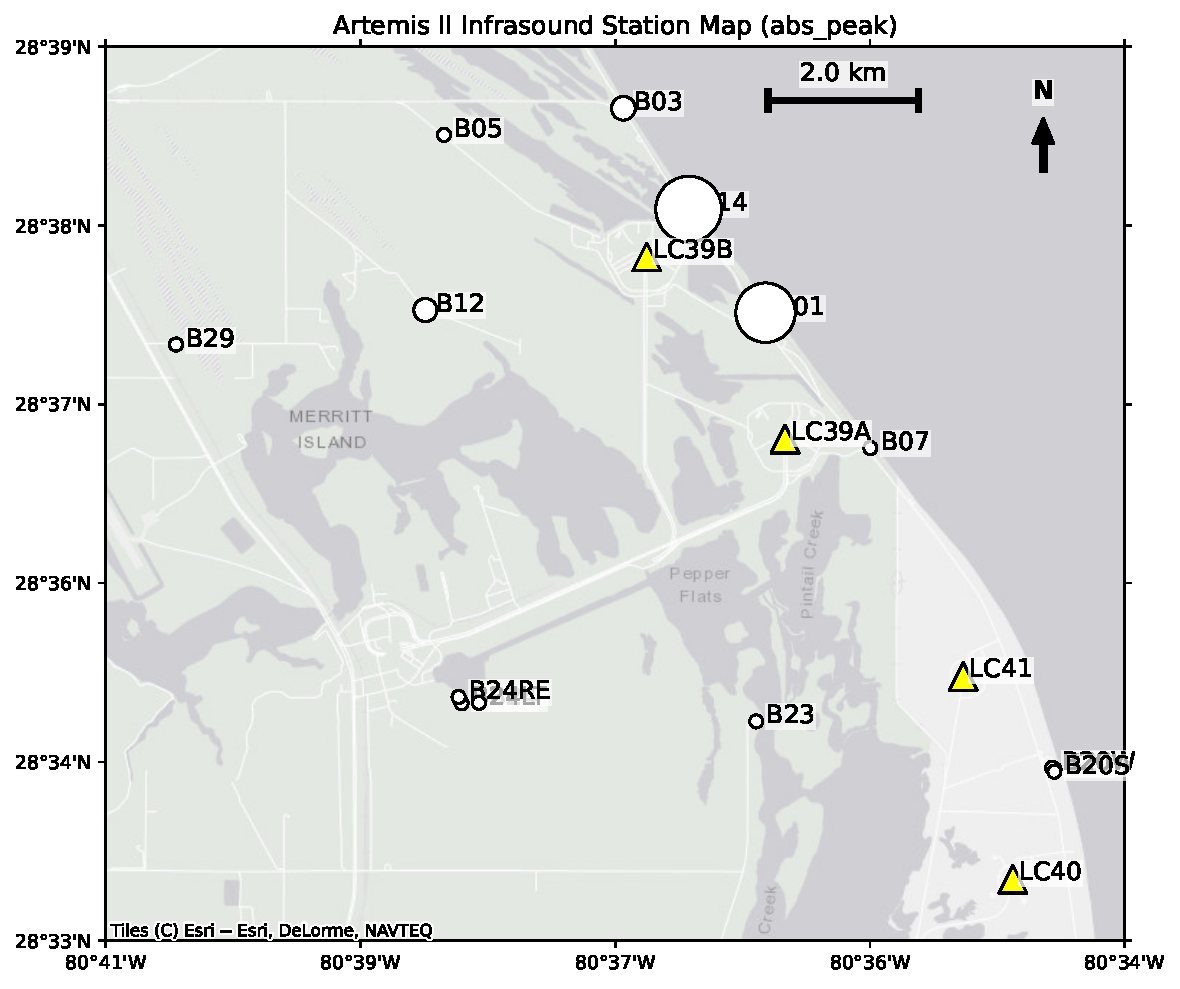
\includegraphics[width=0.95\textwidth]{figures/station_map}
  \caption{Map of infrasound stations (circles) and active launch
    complexes (yellow triangles) for the Artemis~II launch from
    SLC-39B. Station symbols are scaled by peak absolute infrasound
    amplitude. \todo{Regenerate with overflowed Gem channels shown as
    lower bounds (notebook 25).}}
  \label{fig:station_map}
\end{figure}


%% ============================================================
\section{Data and Processing}

\subsection{Data Acquisition and Archiving}
\label{sec:instruments}

At USF broadband sites, Nanometrics Centaur digitizers recorded
continuously to SD cards in the SeisComP Data Structure (SDS), with
daily MiniSEED files for each SEED identifier. The Silicon Audio
accelerometer recorded one-minute MiniSEED files. The G\"{u}ralp
Certimus dataloggers were buried, so only a targeted window around the
launch was retrieved via web interface. Gem data were converted to
MiniSEED with \texttt{gemconvert}. All data were ingested into a single
SDS archive with the \texttt{flovopy.ingest} tools, which validate
each file and map logger serial numbers to SEED identifiers. The Centaurs
label their channels with band code D; we use the SEED band code for
broadband sensors at 250--999 samples per second, C (\texttt{CHZ} for the
Trillium vertical, \texttt{CD0} for the infraBSU), as in the station
metadata. The archive will be deposited with EarthScope.

One channel was damaged in archiving: the B29 vertical (1R.B29.00.CHZ)
day files for 2026 days 082--093 contain only zero bytes in every copy
of the archive. The launch window was recovered exactly from an extract
written on 8~April; the recovery reproduces two intact channels sample
for sample.

\subsection{Instrument Correction}
\label{sec:response}

Waveforms were processed with ObsPy \citep{Beyreuther2010} over a window
from 30~minutes before to 45~minutes after the launch (22:35:12~UTC on
1~April~2026).

\begin{itemize}
  \item \textit{Trillium Compact seismometers and infraBSU
    microbarometers.} Each Centaur writes a StationXML response file
    whenever its configuration changes; we used the latest file written
    before the launch for each station. These files hold the full
    Trillium Compact response (Sensor~A, 40~V$_\text{pp}$;
    $2.995\times10^{8}$~counts per m~s$^{-1}$). For the infraBSU
    channels (Sensor~B, 1~V$_\text{pp}$) the files contain only the
    digitizer, so we prepended the infraBSU sensor stage
    (\SI{46}{\micro\volt\per\pascal}, one high-pass pole at 0.048~Hz),
    giving 735.2~counts~Pa$^{-1}$. Configurations were identical at all
    stations. Pre-filter corners were 0.01, 0.02,
    0.94\,$f_\text{Nyq}$ and 0.98\,$f_\text{Nyq}$.
  \item \textit{Gem infrasound loggers.} Corrected to pressure with the
    \texttt{gemlog} high-gain response after a 0.05~Hz high-pass, and
    after repair of overflow intervals (Section~\ref{sec:overflow}).
  \item \textit{SmartSolo nodes.} The harvested MiniSEED is the
    geophone output voltage in mV, not ground velocity
    (Section~\ref{sec:nodal_validation}). We removed a nominal geophone
    response (5~Hz, damping 0.7, 76.7~V~m$^{-1}$~s) with a pre-filter
    of 0.5--1~Hz at the low end, so SmartSolo results are used only
    above 1~Hz.
  \item \textit{G\"{u}ralp Certimus and Silicon Audio.} Response files
    exist for both Certimus stations, but the B12 response gives
    amplitudes $\sim$10 times higher than neighbouring sensors and was
    written two weeks before the launch configuration; these channels
    are not used quantitatively here.
\end{itemize}

Unconnected digitizer inputs (CD1 and CD2 at B03, B05 and B29) and
channels with no launch signal were identified from their spectral
ratios (Section~\ref{sec:snr}) and removed.

\subsection{Gem Overflow: Detection and Repair}
\label{sec:overflow}

Close to the pad the launch exceeded the Gems' 16-bit range. While a
Gem overflows, consecutive raw samples jump by more than 20{,}000~counts
and the baseline then walks off by $6.6\times10^{4}$ to
$2\times10^{6}$~counts, a step that persists after the overflow. Steep
shock fronts in the signal produce one-sample jumps of similar size
(for example $-71$ to $+122$~Pa within 4~ms at B29, 38.7~s after
launch, recorded by the co-located 500~samples~s$^{-1}$ infraBSU) but leave no persistent step.
We therefore cluster large jumps (2~s gap) and classify each cluster by
the median baseline offset across it: an offset larger than
32{,}768~counts marks an overflow interval (or, for a single jump, a
baseline reset), and smaller offsets mark shocks, which are real signal
and are kept. Overflow intervals, padded by 0.25~s, are masked in all
analyses. Before instrument correction each interval is bridged by a
straight line and the baseline step is removed from the samples after
it; without this repair the step leaks through the 0.05~Hz high-pass as
a slow swing of 120--610~Pa that stays above 10~Pa for 20--37~s after
the interval (largest at B01, $-613$ to $+161$~Pa).

\subsection{Amplitude and Spectral Metrics}

Peak amplitudes are measured in the first 180~s after launch over
unmasked samples only, after a 0.5~Hz (pressure) or 1~Hz (ground
velocity) high-pass, choices justified in Section~\ref{sec:bandwidth}.
Peak level is expressed as $L_\text{pk} =
20\log_{10}(p_\text{pk}/\SI{20}{\micro\pascal})$. Spectra are Welch
estimates over a 180~s launch window and a pre-launch noise window of
equal length, 15~minutes before launch.

\subsection{Software and Reproducibility}
\label{sec:software}

The processing uses ObsPy \citep{Beyreuther2010,krischer_obspy_2015}
and two Python packages: \texttt{ksclib}, shared by our Kennedy Space
Center launch analyses (station metadata, data access, instrument
correction and launch windows), and FlovoPy \citep{flovopy_2026}, whose
\texttt{flovopy.ingest.gem\_overflow} module detects and repairs Gem
overflow (Section~\ref{sec:overflow}). The analysis is a sequence of
Jupyter notebooks. Notebooks 20--60, run in order, compute every result
and write it to CSV files and figures; notebook 65 writes the tables in
this paper from those files; and a script (\texttt{compose\_figures.py})
copies each figure from the notebook outputs. Every table and figure can
therefore be regenerated from the waveform archive (see Data and Code
Availability).


\subsection{Overview of the Recordings}
\label{sec:overview}

Figure~\ref{fig:overview} shows the corrected launch records for every
pressure and vertical-velocity channel, sorted by distance, with the
B01 spectrograms. Sound from the pad reaches B14 (0.7~km) a few seconds
before liftoff, from the start of the core-stage engines (\papertwo), and
the B20 cluster (7.6~km) $\sim$22~s after liftoff.
The strongest pressure arrives 20--40~s after liftoff at most stations
and $\sim$40--75~s at the farthest, and lasts for 1--2~minutes; peak
pressures range from 512~Pa at B01 (1.5~km) to 42--45~Pa at 7.6~km, and
peak vertical velocities from 7.5~mm~s$^{-1}$ at B14 to
0.5~mm~s$^{-1}$ at B20. The ground motion follows the pressure closely
in timing at every site. The Gem overflow intervals
(Section~\ref{sec:clipping}) appear as gaps in the closest Gem records,
and at B03 and B05, north of the pad, the strongest pressure arrives in
the first $\sim$10~s. At B01 both pressure and ground motion extend to
the top of the 500~samples~s$^{-1}$ band, and their high frequencies
decline as the vehicle climbs.

\begin{figure}[htbp]
  \centering
  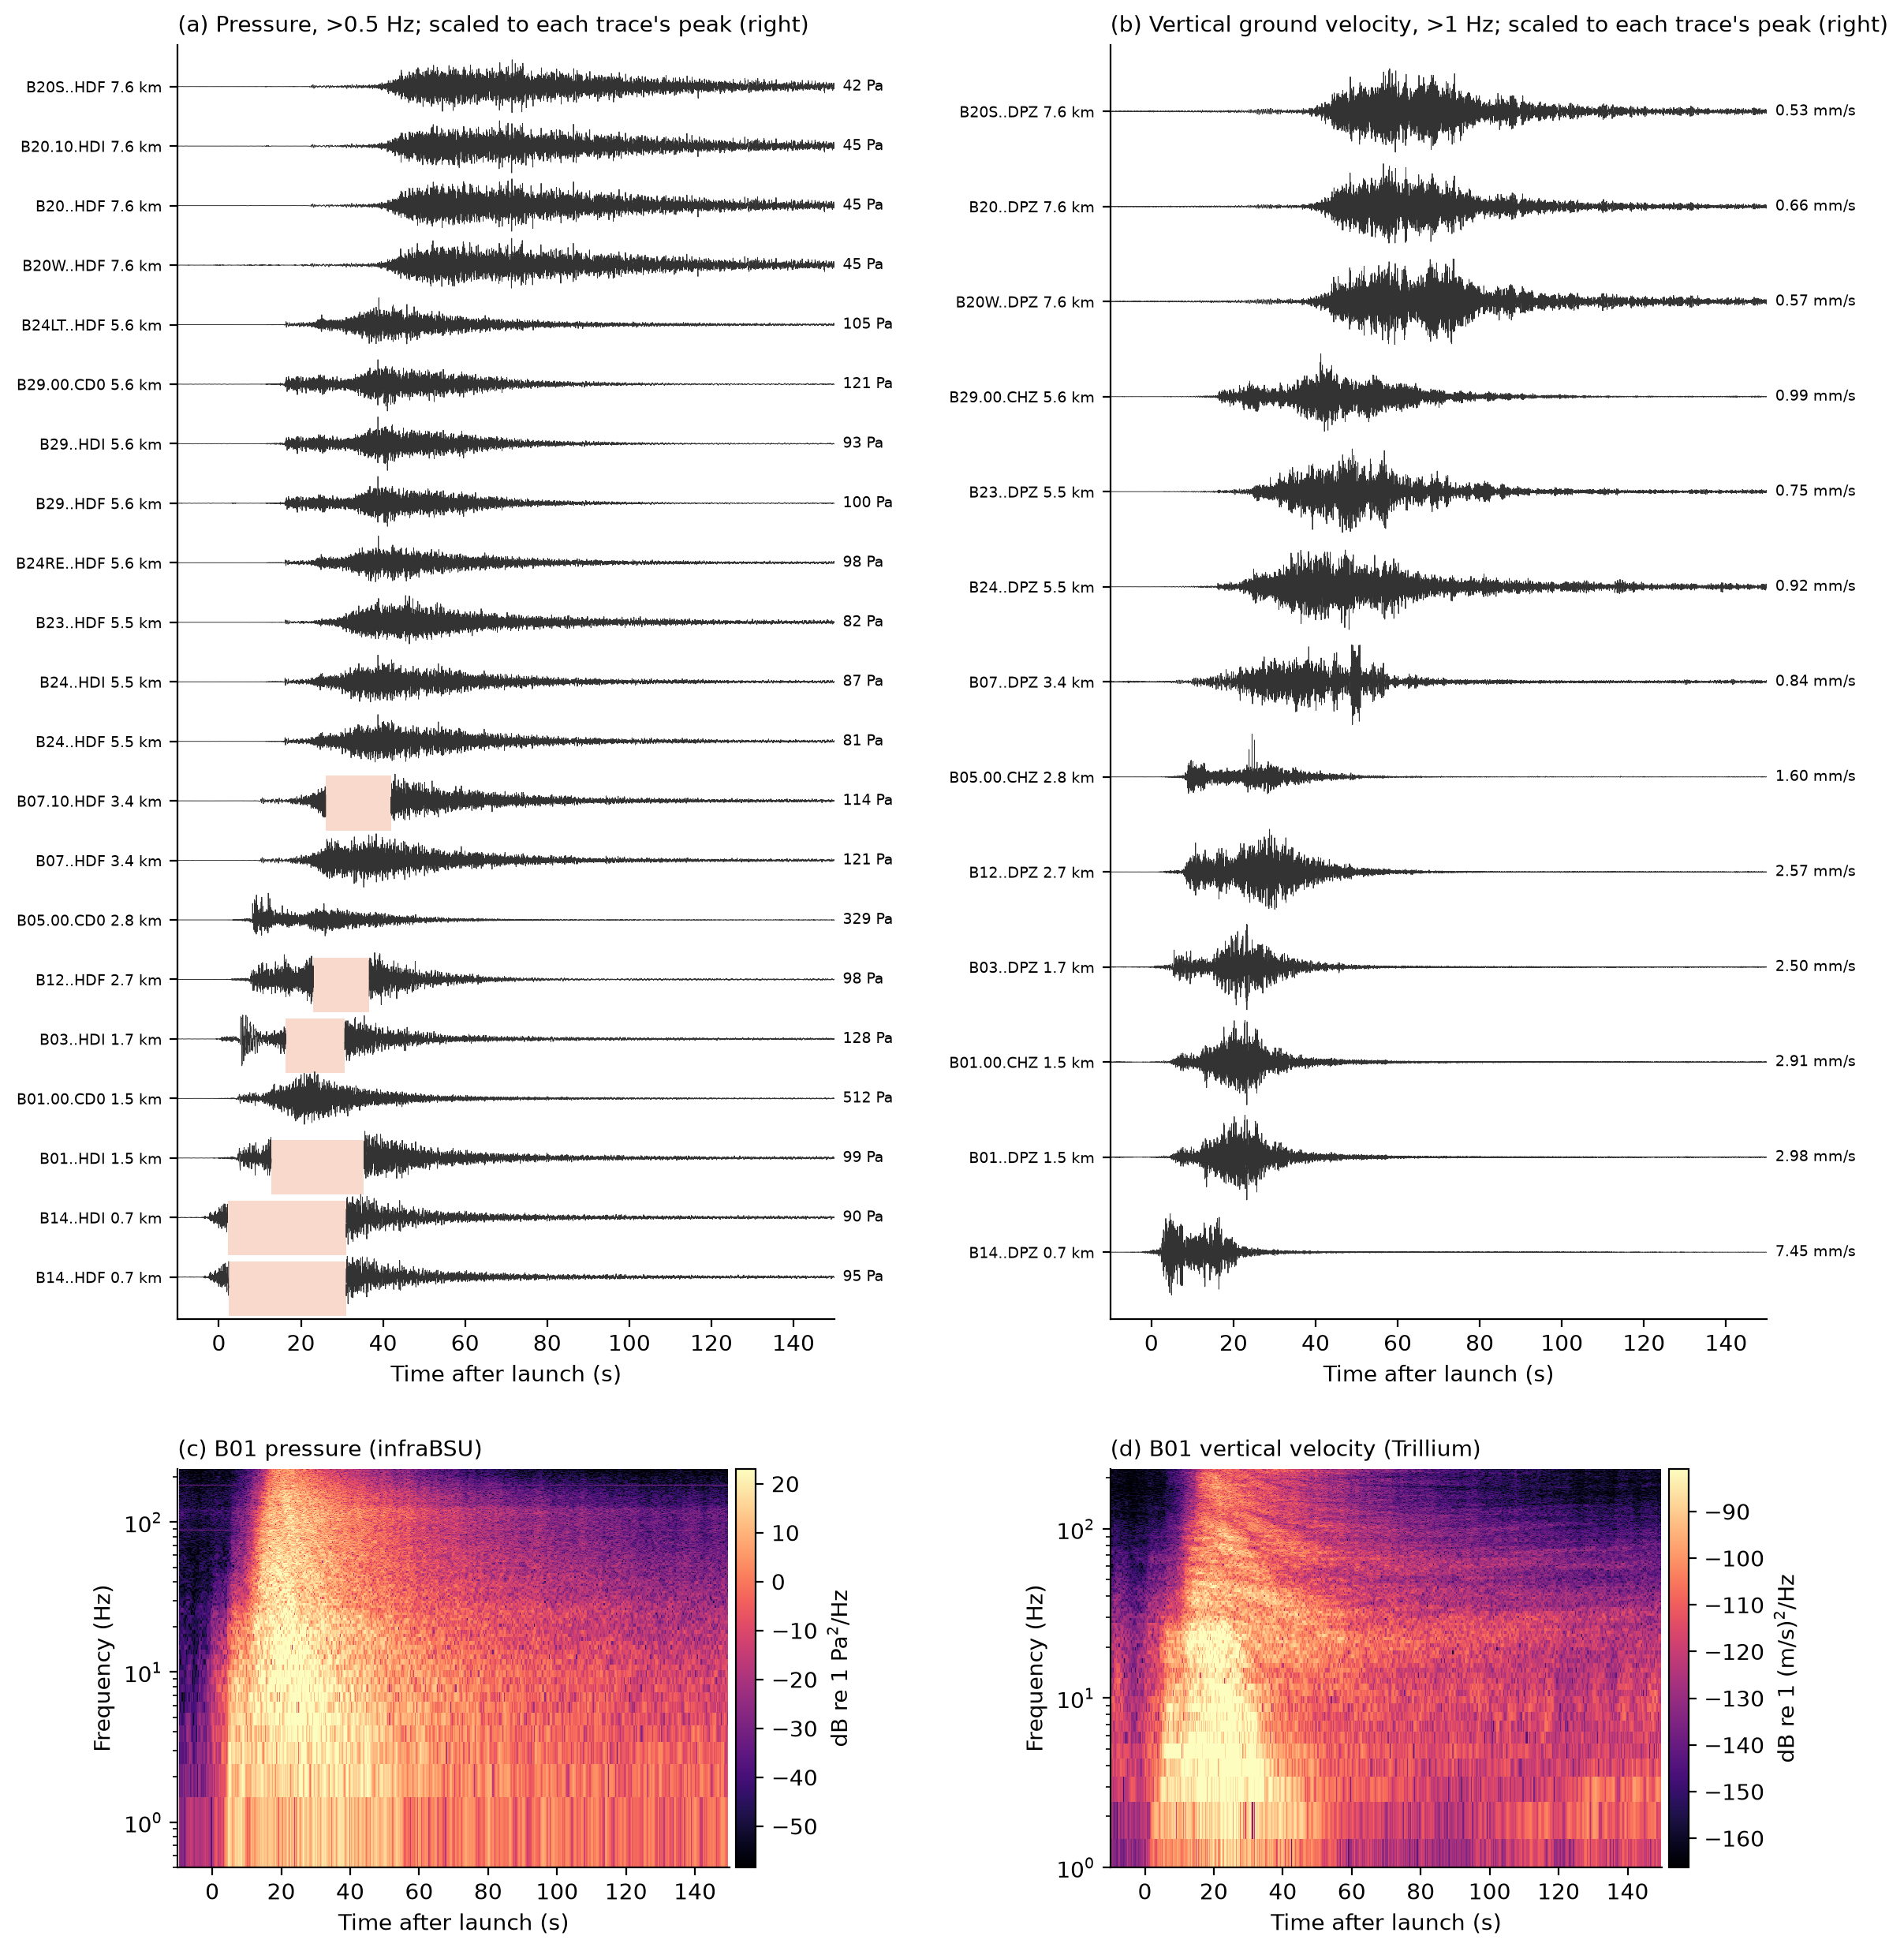
\includegraphics[width=\textwidth]{data_overview}
  \caption{The Artemis~II launch across the network. (a) Pressure
    ($>$0.5~Hz; infraBSU and Gem) and (b) vertical ground velocity
    ($>$1~Hz; Trillium and SmartSolo, the latter sign-corrected) for every
    channel, sorted by distance from SLC-39B and each scaled to its own
    peak (value at right, at the native sampling rate; display decimated to
    100~samples~s$^{-1}$). Orange: Gem overflow intervals (blanked). B03's
    faulty Centaur channels are omitted. (c, d) Spectrograms of pressure and
    vertical velocity at B01 (1.5~km).}
  \label{fig:overview}
\end{figure}

%% ============================================================
\section{Network Validation and Data Quality}
\label{sec:observations}

\subsection{Station Performance}
\label{sec:quality}

Of the seven USF Centaur stations, four (B01, B03, B05 and B29) recorded
the launch. The Centaurs at B14, B20 and B24 have no data on launch day
(B20's record resumes on 4~April), so the Chaparral sensor at B20
produced no launch record; the co-located Gems and SmartSolos at those
sites did record.

No Centaur channel approached full scale during the launch: the
largest was B01 CHZ at 10\% of the 24-bit range. B03 recorded the launch
on all channels but far too low: its seismometer's peak velocity is
$\sim$35 times below that of the co-located SmartSolo, and its infraBSU
peak at least $\sim$50 times below that of the co-located Gem, although
its configuration was identical to the other stations; we attribute this to a hardware fault
in the B03 digitizer and exclude its Centaur channels. At B05 the
Trillium's horizontal channels sat at 79\% and 98\% of full scale
before the launch, indicating an off-centre sensor mass. B05's vertical
drifts by $\sim$1~mm~s$^{-1}$ over minutes from before the launch; its
seismic channels are used only above 1~Hz and excluded from fits.

\subsection{Infrasound Clipping}
\label{sec:clipping}

Six Gem channels overflowed during the launch
(Figure~\ref{fig:clipping}): B14~HDF and HDI (0.7~km; 2--31~s after
launch), B01~HDI (1.5~km; 13--35~s), B03~HDI (1.7~km; 16--31~s), B12~HDF
(2.7~km; 23--37~s) and B07.10~HDF (3.4~km; 26--42~s, a single
wraparound). Gems at 5.5~km and beyond did not overflow, although
several recorded individual shock fronts large enough to resemble
overflow in the raw counts. Comparison with the infraBSU at B01 shows
that the Gem begins to overflow when pressure reaches
$\sim$100--140~Pa at high gain.

The co-located infraBSU at B01 also validates the Gem record outside
the overflow interval (Figure~\ref{fig:clipping}b). In 5-s windows outside the
interval, the corrected Gem and infraBSU waveforms correlate at 0.99
(1--20~Hz) with an RMS amplitude ratio of 0.96; after the repair, the
broadband (0.05--40~Hz) correlation is 0.94--0.95 from the end of the
interval to 120~s after launch, and 0.93 from 120 to 300~s. Below 1~Hz
a residual of the overflow persists for $\sim$15~s after the interval:
the 0.05--1~Hz correlation in 10-s windows is 0.62 just after it and
first exceeds 0.8 about 16~s after it. Overflowed
Gems therefore remain usable before and after their overflow
intervals, above $\sim$0.5~Hz, and we retain them in all analyses with
the intervals masked.

\begin{figure}[htbp]
  \centering
  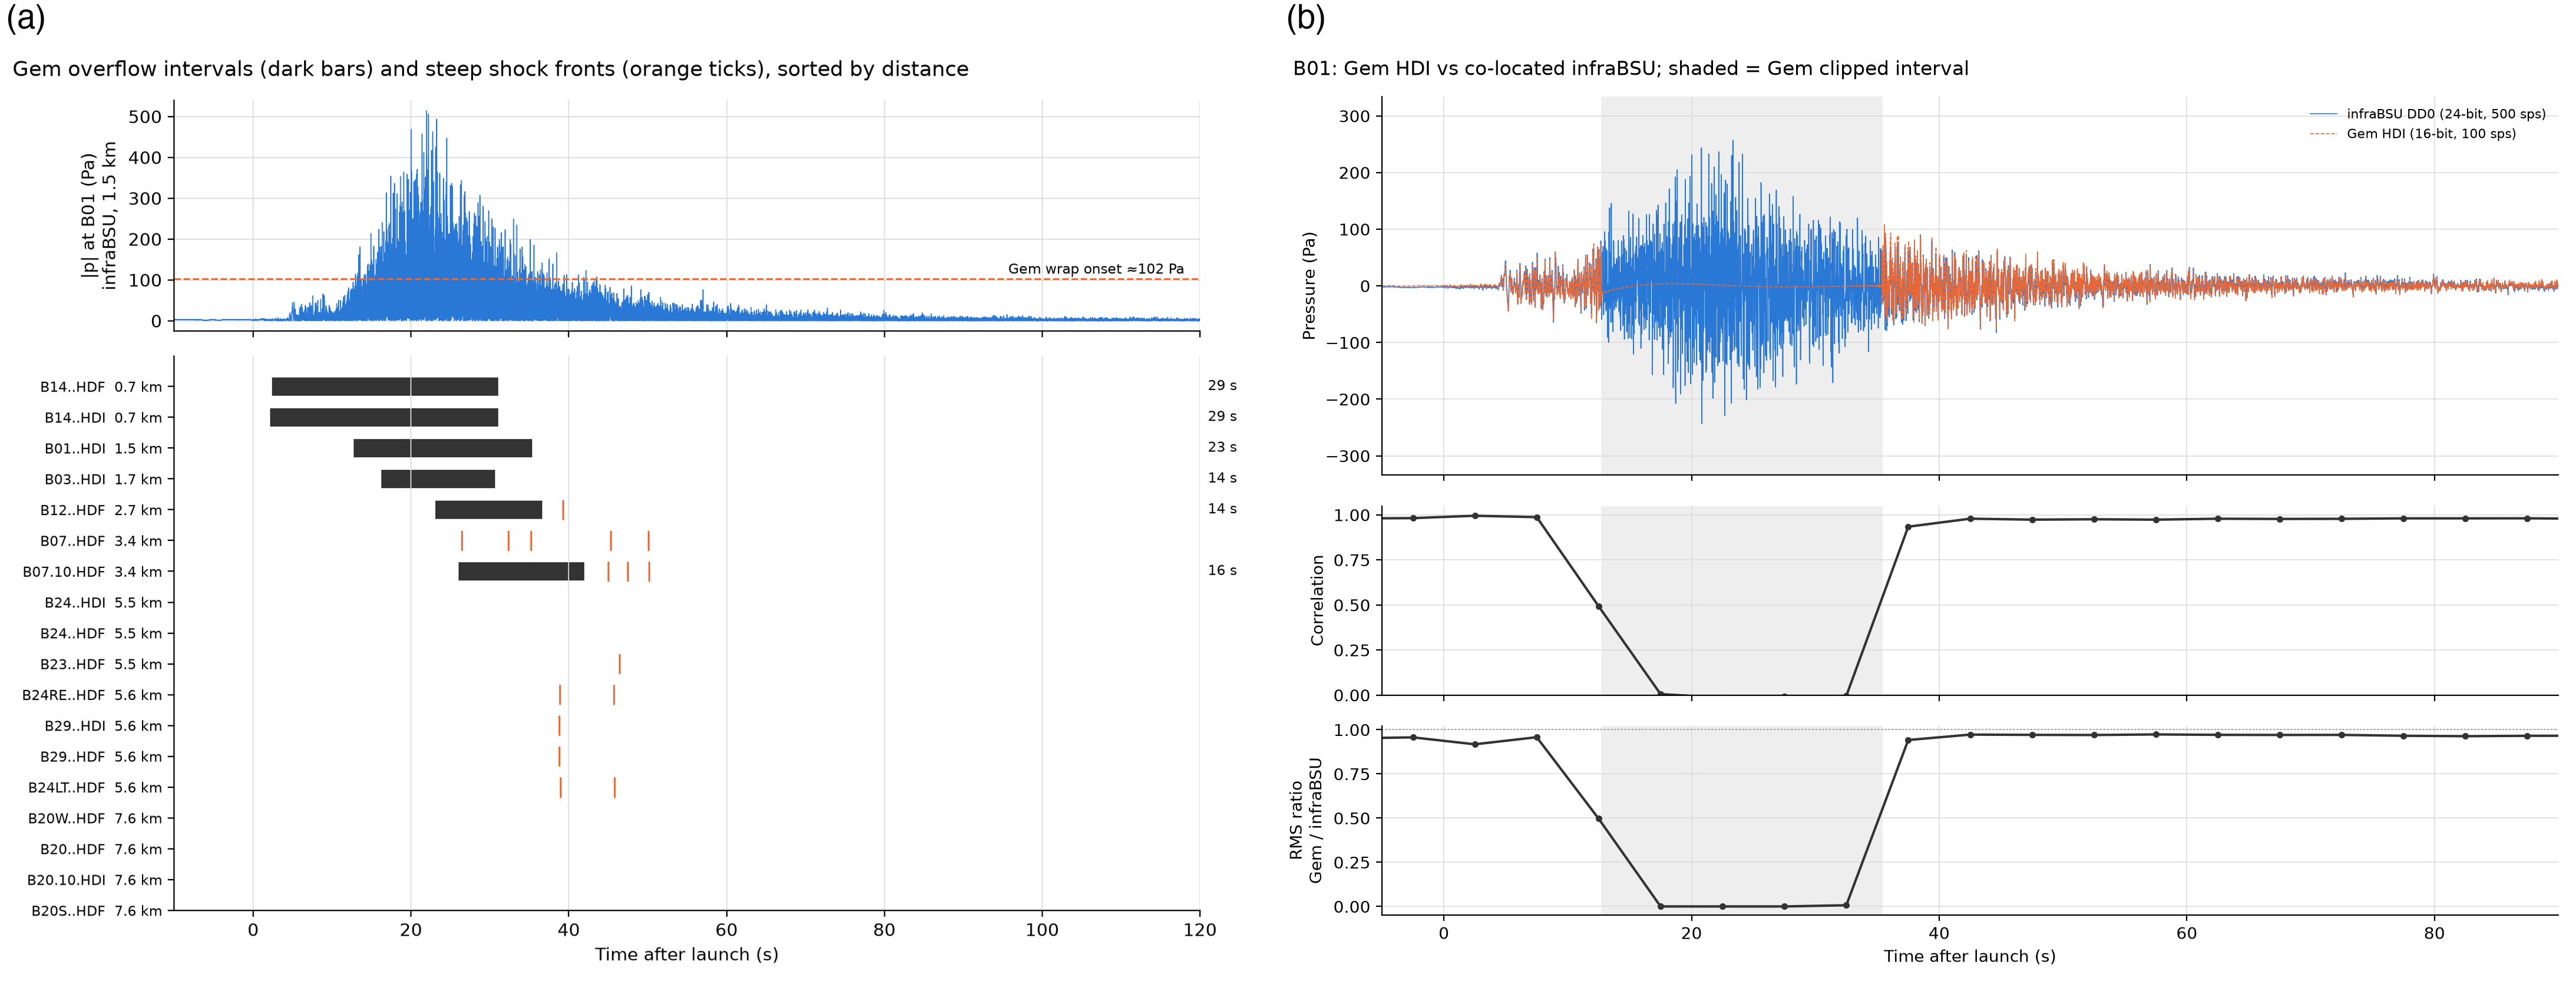
\includegraphics[width=\textwidth]{composite_overflow}
  \caption{Gem overflow during the launch. (a) Top: absolute pressure at
    B01 (infraBSU, 1.5~km), with the pressure at which the B01 Gem began to
    overflow (dashed). Bottom: overflow intervals (dark bars, with total
    duration at right) and steep shock fronts that are not overflow (orange
    ticks) for every Gem, sorted by distance from SLC-39B. (b) Validation at
    B01: corrected pressure from the infraBSU and the co-located Gem after
    overflow repair (shaded: the Gem's overflow interval, bridged), with
    their correlation and RMS ratio in 5-s windows (1--20~Hz).}
  \label{fig:clipping}
\end{figure}

\subsection{Broadband--Nodal Comparison at Co-located Sites}
\label{sec:nodal_validation}

At B01, where a SmartSolo node sits beside a working Trillium Compact,
the spectral ratio of the raw SmartSolo record to the Trillium velocity
levels off at 74{,}000~mV per m~s$^{-1}$ above $\sim$10~Hz, close to
the nominal geophone sensitivity (76{,}700), and rolls off below 5~Hz
with a $90^{\circ}$ phase shift at 5~Hz (Figure~\ref{fig:smartsolo}).
The harvested SmartSolo data are therefore geophone output voltage and
require the geophone response to be removed. After correction, the
SmartSolo and Trillium peak velocities at B01 agree within 4\% (1--100~Hz;
\suppfig{2}), and the peak vertical velocities at B01 are 2.98 and 2.91~mm~s$^{-1}$;
across the network, SmartSolo and Trillium peak ground velocities fall on a
single trend with distance (\papertwo).

The SmartSolo vertical has reversed polarity relative to the Trillium
(zero-lag correlation $-0.94$). The air-to-ground coupling
(Section~\ref{sec:coupling}) shows which is standard: compression should
push the ground down, and the Trillium verticals at B01 and B29 indeed
correlate negatively with pressure, whereas the SmartSolo verticals
correlate positively at every site except B03 (Table~\ref{tab:coupling}).
The SmartSolo verticals are therefore reversed
with respect to the up-positive convention; their sign is flipped in
waveform comparisons. The polarity of the horizontal components has not
been checked.

\begin{figure}[htbp]
  \centering
  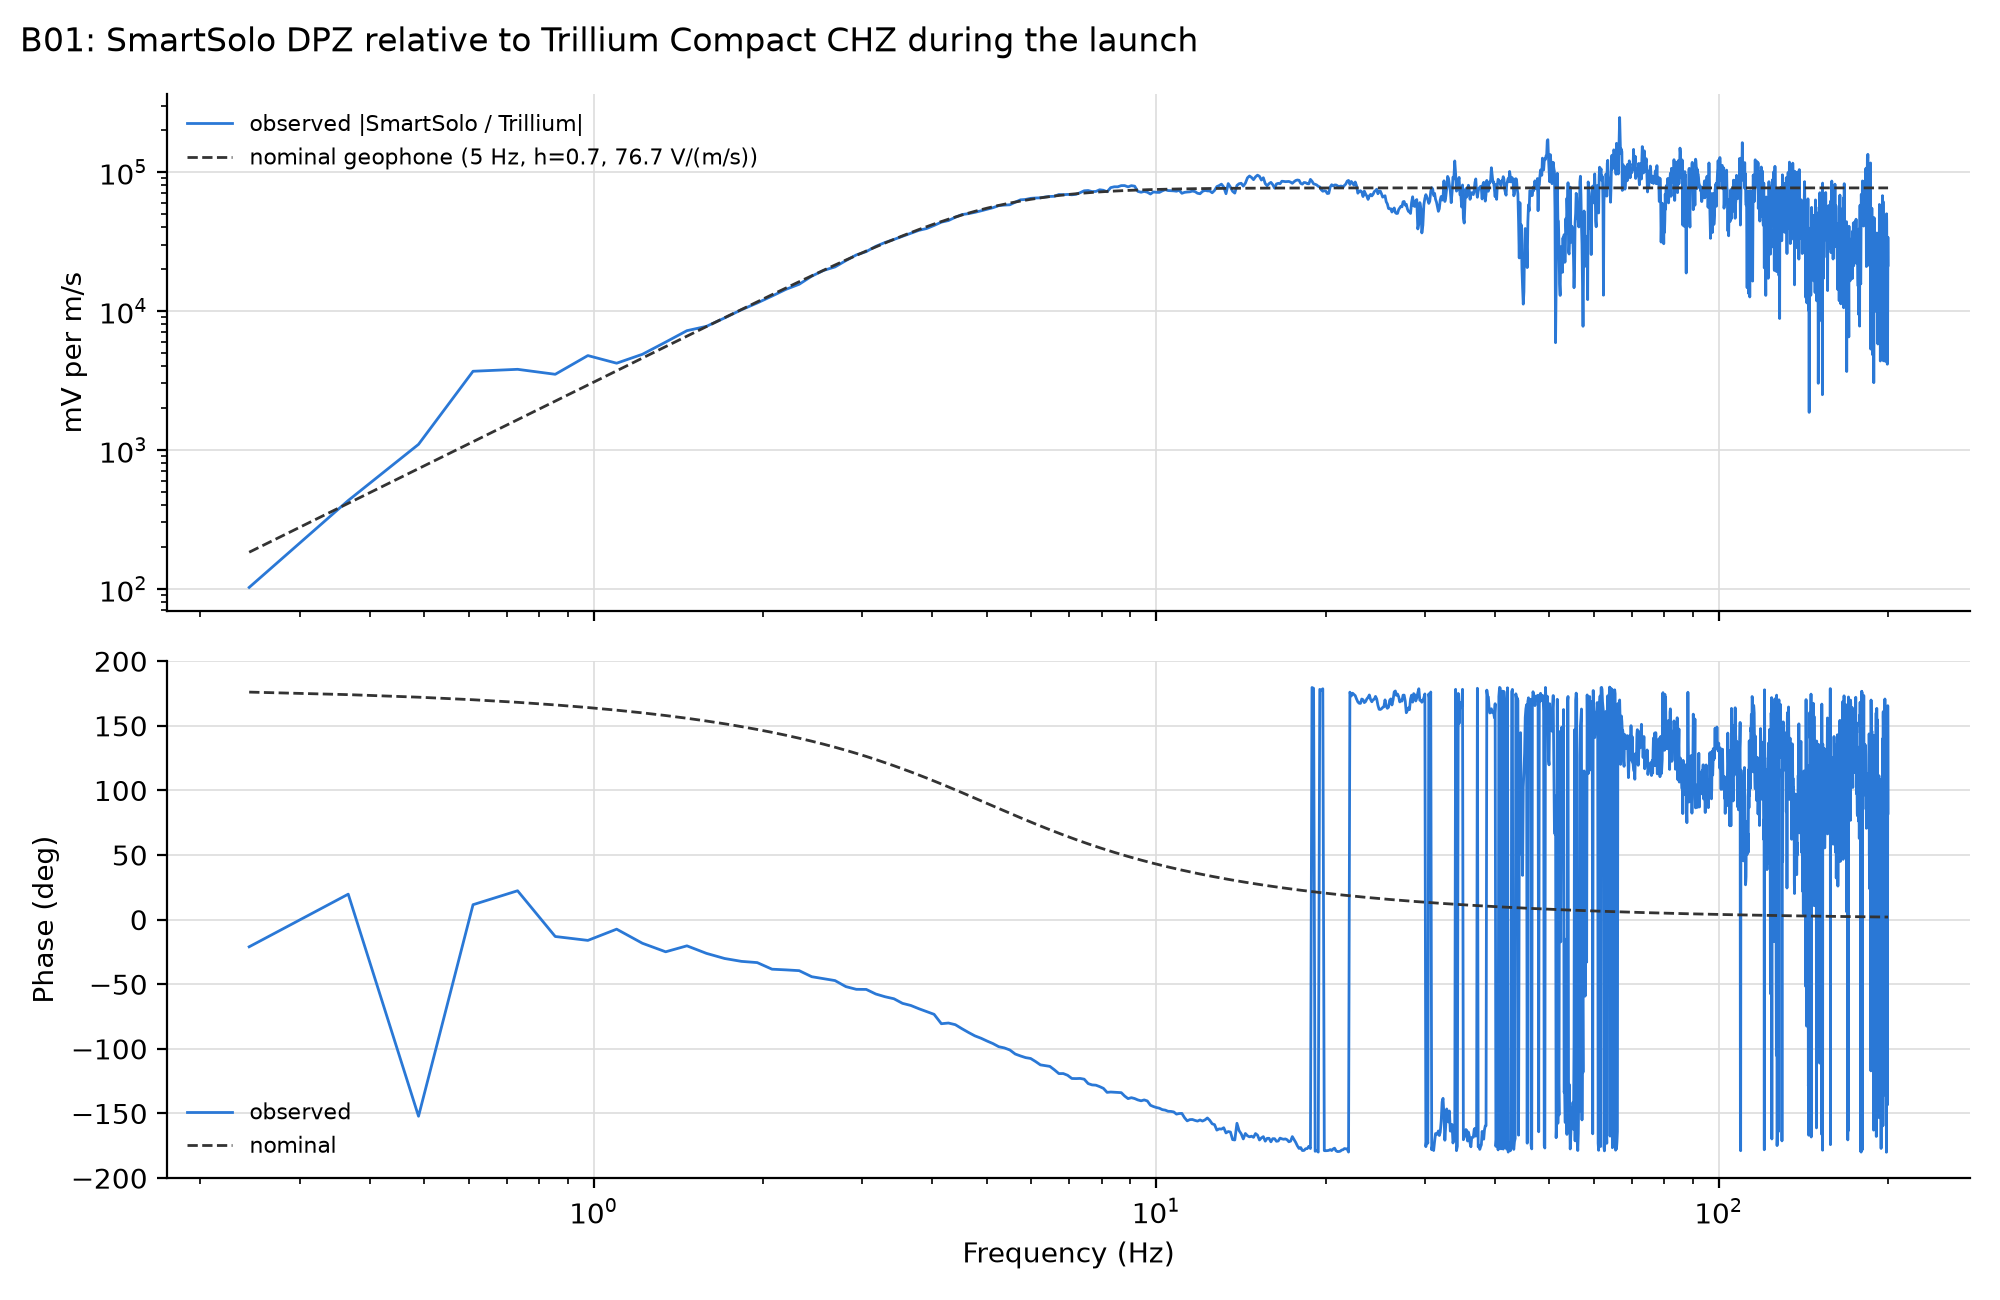
\includegraphics[width=0.85\textwidth]{smartsolo_vs_trillium_B01_transfer}
  \caption{SmartSolo DPZ (raw, mV) relative to Trillium Compact CHZ
    velocity at B01 during the launch: amplitude and phase of the
    transfer function, with the nominal 5~Hz geophone response for
    comparison.}
  \label{fig:smartsolo}
\end{figure}

\subsection{Enclosure Effects: Tote versus Free-field Gem Sensors}
\label{sec:enclosure}

Three tote--free-field pairs were usable (at B14 both overflowed and at
B03 the free-field Gem stopped before launch); the Gems in each pair were
3--6~m apart. In broadband terms the tote and free-field records are
nearly indistinguishable: peak ratios HDI/HDF are 1.05 (B20), 1.08 (B24)
and 0.94 (B29), RMS ratios 0.96--1.04, and coherence 0.998--0.999 over
0.5--20~Hz (Figure~\ref{fig:enclosure}a; example pair in \suppfig{1}). Coherence remains above 0.98
when the band is extended to 45~Hz (0.9 times the Nyquist frequency),
and RMS ratios remain within 0.96--1.06 for any upper limit from 20 to
45~Hz, because most launch energy at the Gems lies below 20~Hz. In
separate frequency bands, however, the totes alter the spectrum above
$\sim$10~Hz (Figure~\ref{fig:enclosure}b): at B20 the tote record is 1.1~dB higher
at 10--20~Hz and 2.4--4.2~dB lower at 20--45~Hz, at B29 it is
0.4--0.9~dB lower above 10~Hz, and at B24 0.2--1.2~dB higher. For
comparison, two free-field Gems 9~m apart at B20 agree within 0.2~dB in
every band up to 45~Hz, whereas free-field Gems 30--36~m apart differ by
up to 1.3~dB below 40~Hz and lose coherence (0.2--0.5 above 10~Hz),
which sets the useful band of the B20 array. Before the launch, the tote
reduced noise at B29 (median PSD ratio 0.33 over 0.5--20~Hz) and B24
(0.74), but not at B20 (1.23). Tote enclosures can therefore be used
without correction for amplitudes, timing and spectra below $\sim$10~Hz,
with a possible gain in wind-noise reduction; above $\sim$10~Hz they
introduce site-dependent spectral changes of up to $\pm$4~dB, which
matter for spectral and crackle analyses.
A simple acoustic model of the 27-gallon HDPE tote (Text~S1) explains
this pattern. Standing waves in the enclosed air require frequencies
above $\sim$260~Hz, and leakage around the snap-fit lid may produce a
Helmholtz resonance near $\sim$100~Hz, but the bending modes of the
$\sim$2~mm walls begin at $\sim$10--30~Hz. Because the lid alone is
25--55 times more compliant than the enclosed air, the interior pressure follows
the exterior within a few per cent below the panel modes, even with a
sealed lid, so the tote is transparent at low frequencies; above
$\sim$10~Hz panel resonances amplify or attenuate the signal by amounts
that depend on lid fit, leakage and how the tote sits on the ground,
consistent with the site-to-site differences observed.
The infraBSU microbarometers at the Centaur sites were installed in the
same type of tote, which also housed the digitizer, battery and other
electronics. At B29 the infraBSU record is 0.3--0.5~dB below that of the
adjacent free-field Gem below 10~Hz and 1.6--2.9~dB below it at
10--40~Hz; no free-field reference exists above 50~Hz (Text~S1).

\begin{figure}[htbp]
  \centering
  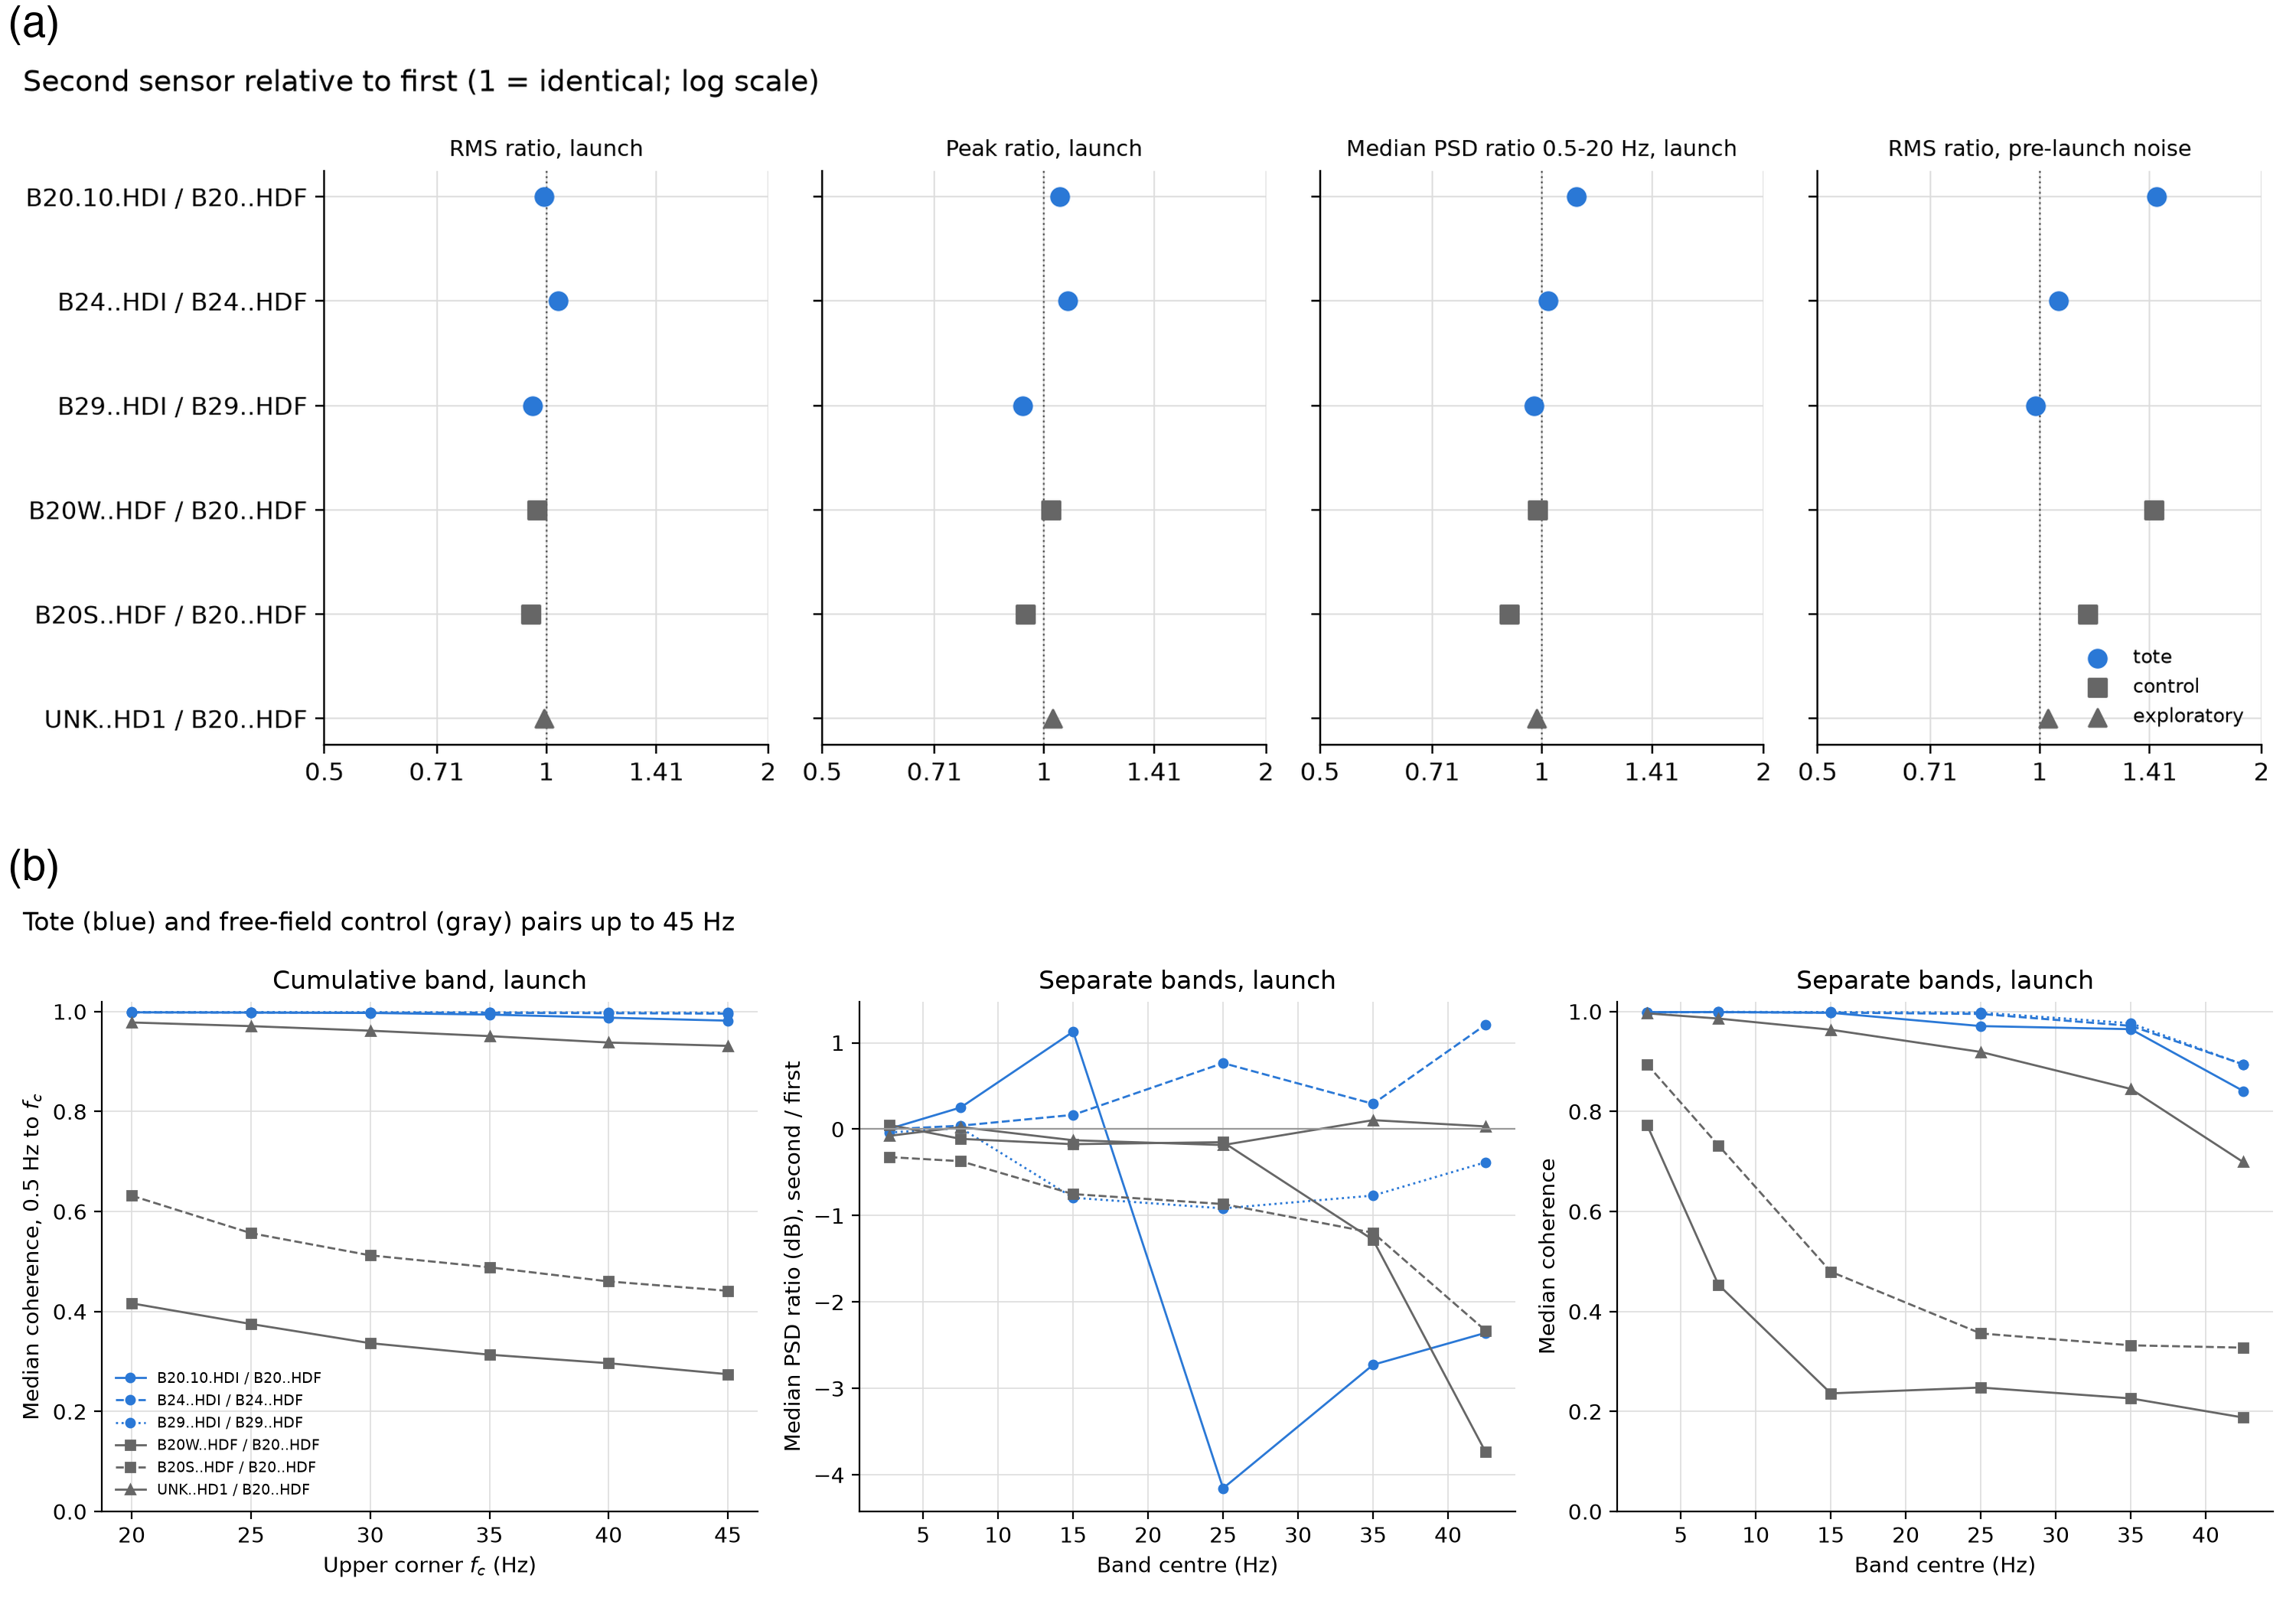
\includegraphics[width=\textwidth]{composite_enclosure}
  \caption{Tote (HDI) versus free-field (HDF) Gem pairs (blue) and free-field
    control pairs at B20 (gray). (a) Second sensor relative to the first: RMS,
    peak and median PSD ratio (0.5--20~Hz) during the launch, and RMS ratio of
    pre-launch noise. (b) Up to 45~Hz: median coherence from 0.5~Hz to an
    upper corner of 20--45~Hz, and median PSD ratio (dB) and coherence in
    separate bands.}
  \label{fig:enclosure}
\end{figure}


%% ============================================================
\section{Signal Bandwidth and Recording Requirements}
\label{sec:bandwidth}

\subsection{Launch-to-Noise Spectral Ratios}
\label{sec:snr}

The ratio of launch to pre-launch power spectral density
(Figure~\ref{fig:snr}) shows where the rocket signal lies. For pressure,
the ratio first exceeds 10 at a median of 0.5~Hz and remains above it to
the top of each sensor's band (45~Hz for the Gems, 225~Hz for the
infraBSUs), peaking at $\sim$13~Hz. For ground velocity the ratio exceeds
10 from $\sim$1~Hz, peaks at a median of 28~Hz and remains high to
225~Hz. Below 0.5~Hz the launch adds almost nothing: on the Centaur
channels at most 0.5\% of the excess pressure energy (launch minus noise)
and at most 0.3\% of the excess seismic energy lies below 0.5~Hz,
whereas 87\% of the pre-launch pressure noise and up to 42\% of the
seismic noise (B29) does. Most rocket energy is in the 1--20~Hz band in
both pressure and ground motion, with 20--50\% above 20~Hz at the near
infraBSUs (\suppfig{4}). A 0.5~Hz high-pass filter therefore removes
background, mostly wind noise and microseisms, without removing launch
signal, and we apply it throughout.

\begin{figure}[htbp]
  \centering
  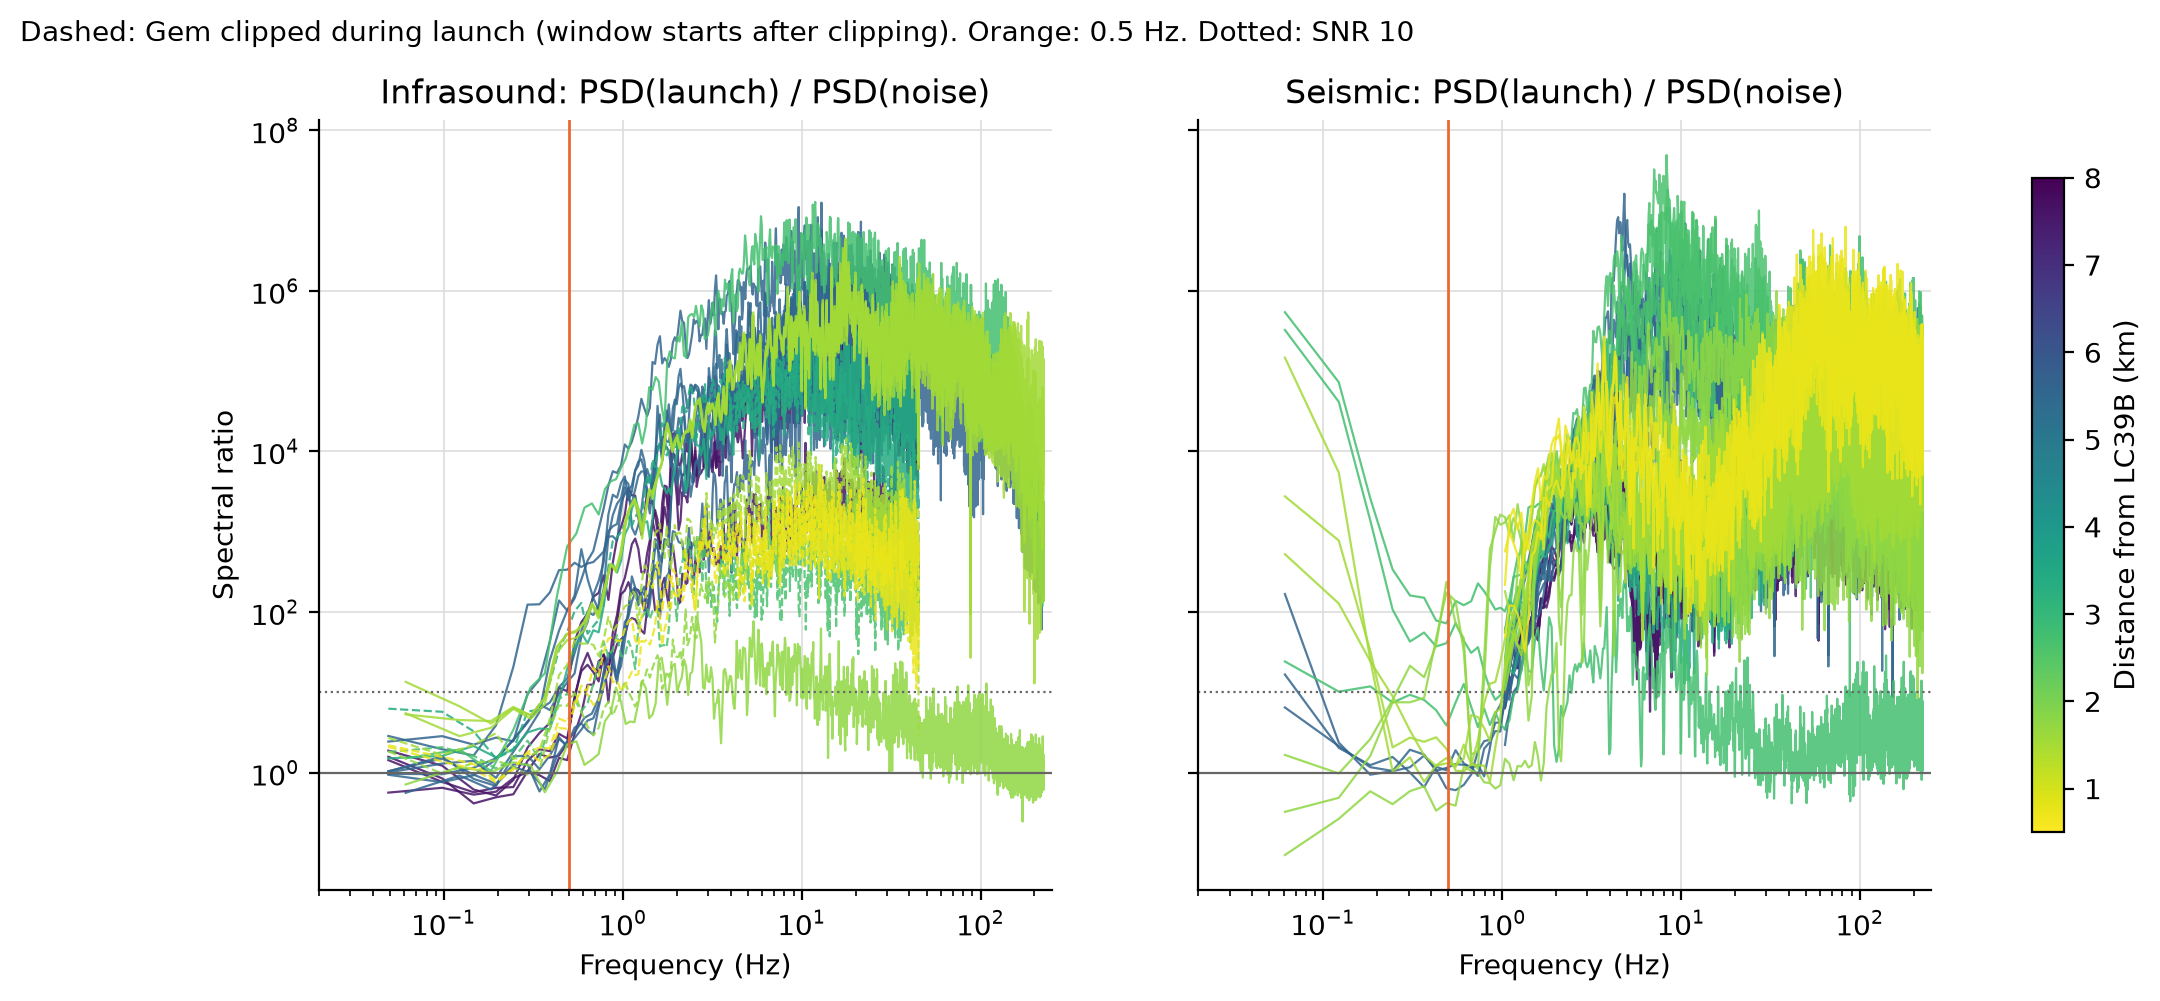
\includegraphics[width=\textwidth]{snr_spectra}
  \caption{Ratio of launch to pre-launch power spectral density for
    every pressure (left) and vertical and horizontal velocity (right)
    channel, coloured by distance from SLC-39B. Dashed: Gems that
    overflowed, with the launch window starting after their overflow.
    Orange line: 0.5~Hz. Dotted line: ratio of 10. SmartSolo spectra are
    shown above 1~Hz only.}
  \label{fig:snr}
\end{figure}

\subsection{Sampling Rate}

We decimated the 500~samples~s$^{-1}$ Centaur records (with
anti-alias filtering) and measured what is lost
(Figure~\ref{fig:bandwidth}a; spectra in \suppfig{3}). For ground velocity at B01 and B29,
250~samples~s$^{-1}$ discards 1--6\% of the rocket energy and retains
97--98\% of the peak; 100~samples~s$^{-1}$ discards 6--10\% and retains
83--92\% of the peak. Pressure near the pad is more demanding: at B01
(1.5~km), 250~samples~s$^{-1}$ discards 11\% of the energy and 19\% of
the peak, and 100~samples~s$^{-1}$, the Gem rate, discards 30\% of the
energy and 43\% of the peak. At 2.8--5.6~km the losses at
100~samples~s$^{-1}$ fall to 11--14\% of the energy. Consistent with
this, the Gems at B29 record peak pressures $\sim$20\% below the
co-located infraBSU (93--100 versus 121~Pa). Measures of crackle are even more sensitive to sampling rate: the skewness of
the pressure derivative at 100~samples~s$^{-1}$ is only $\sim$40\% of its
500~samples~s$^{-1}$ value (\papertwo).

\begin{figure}[htbp]
  \centering
  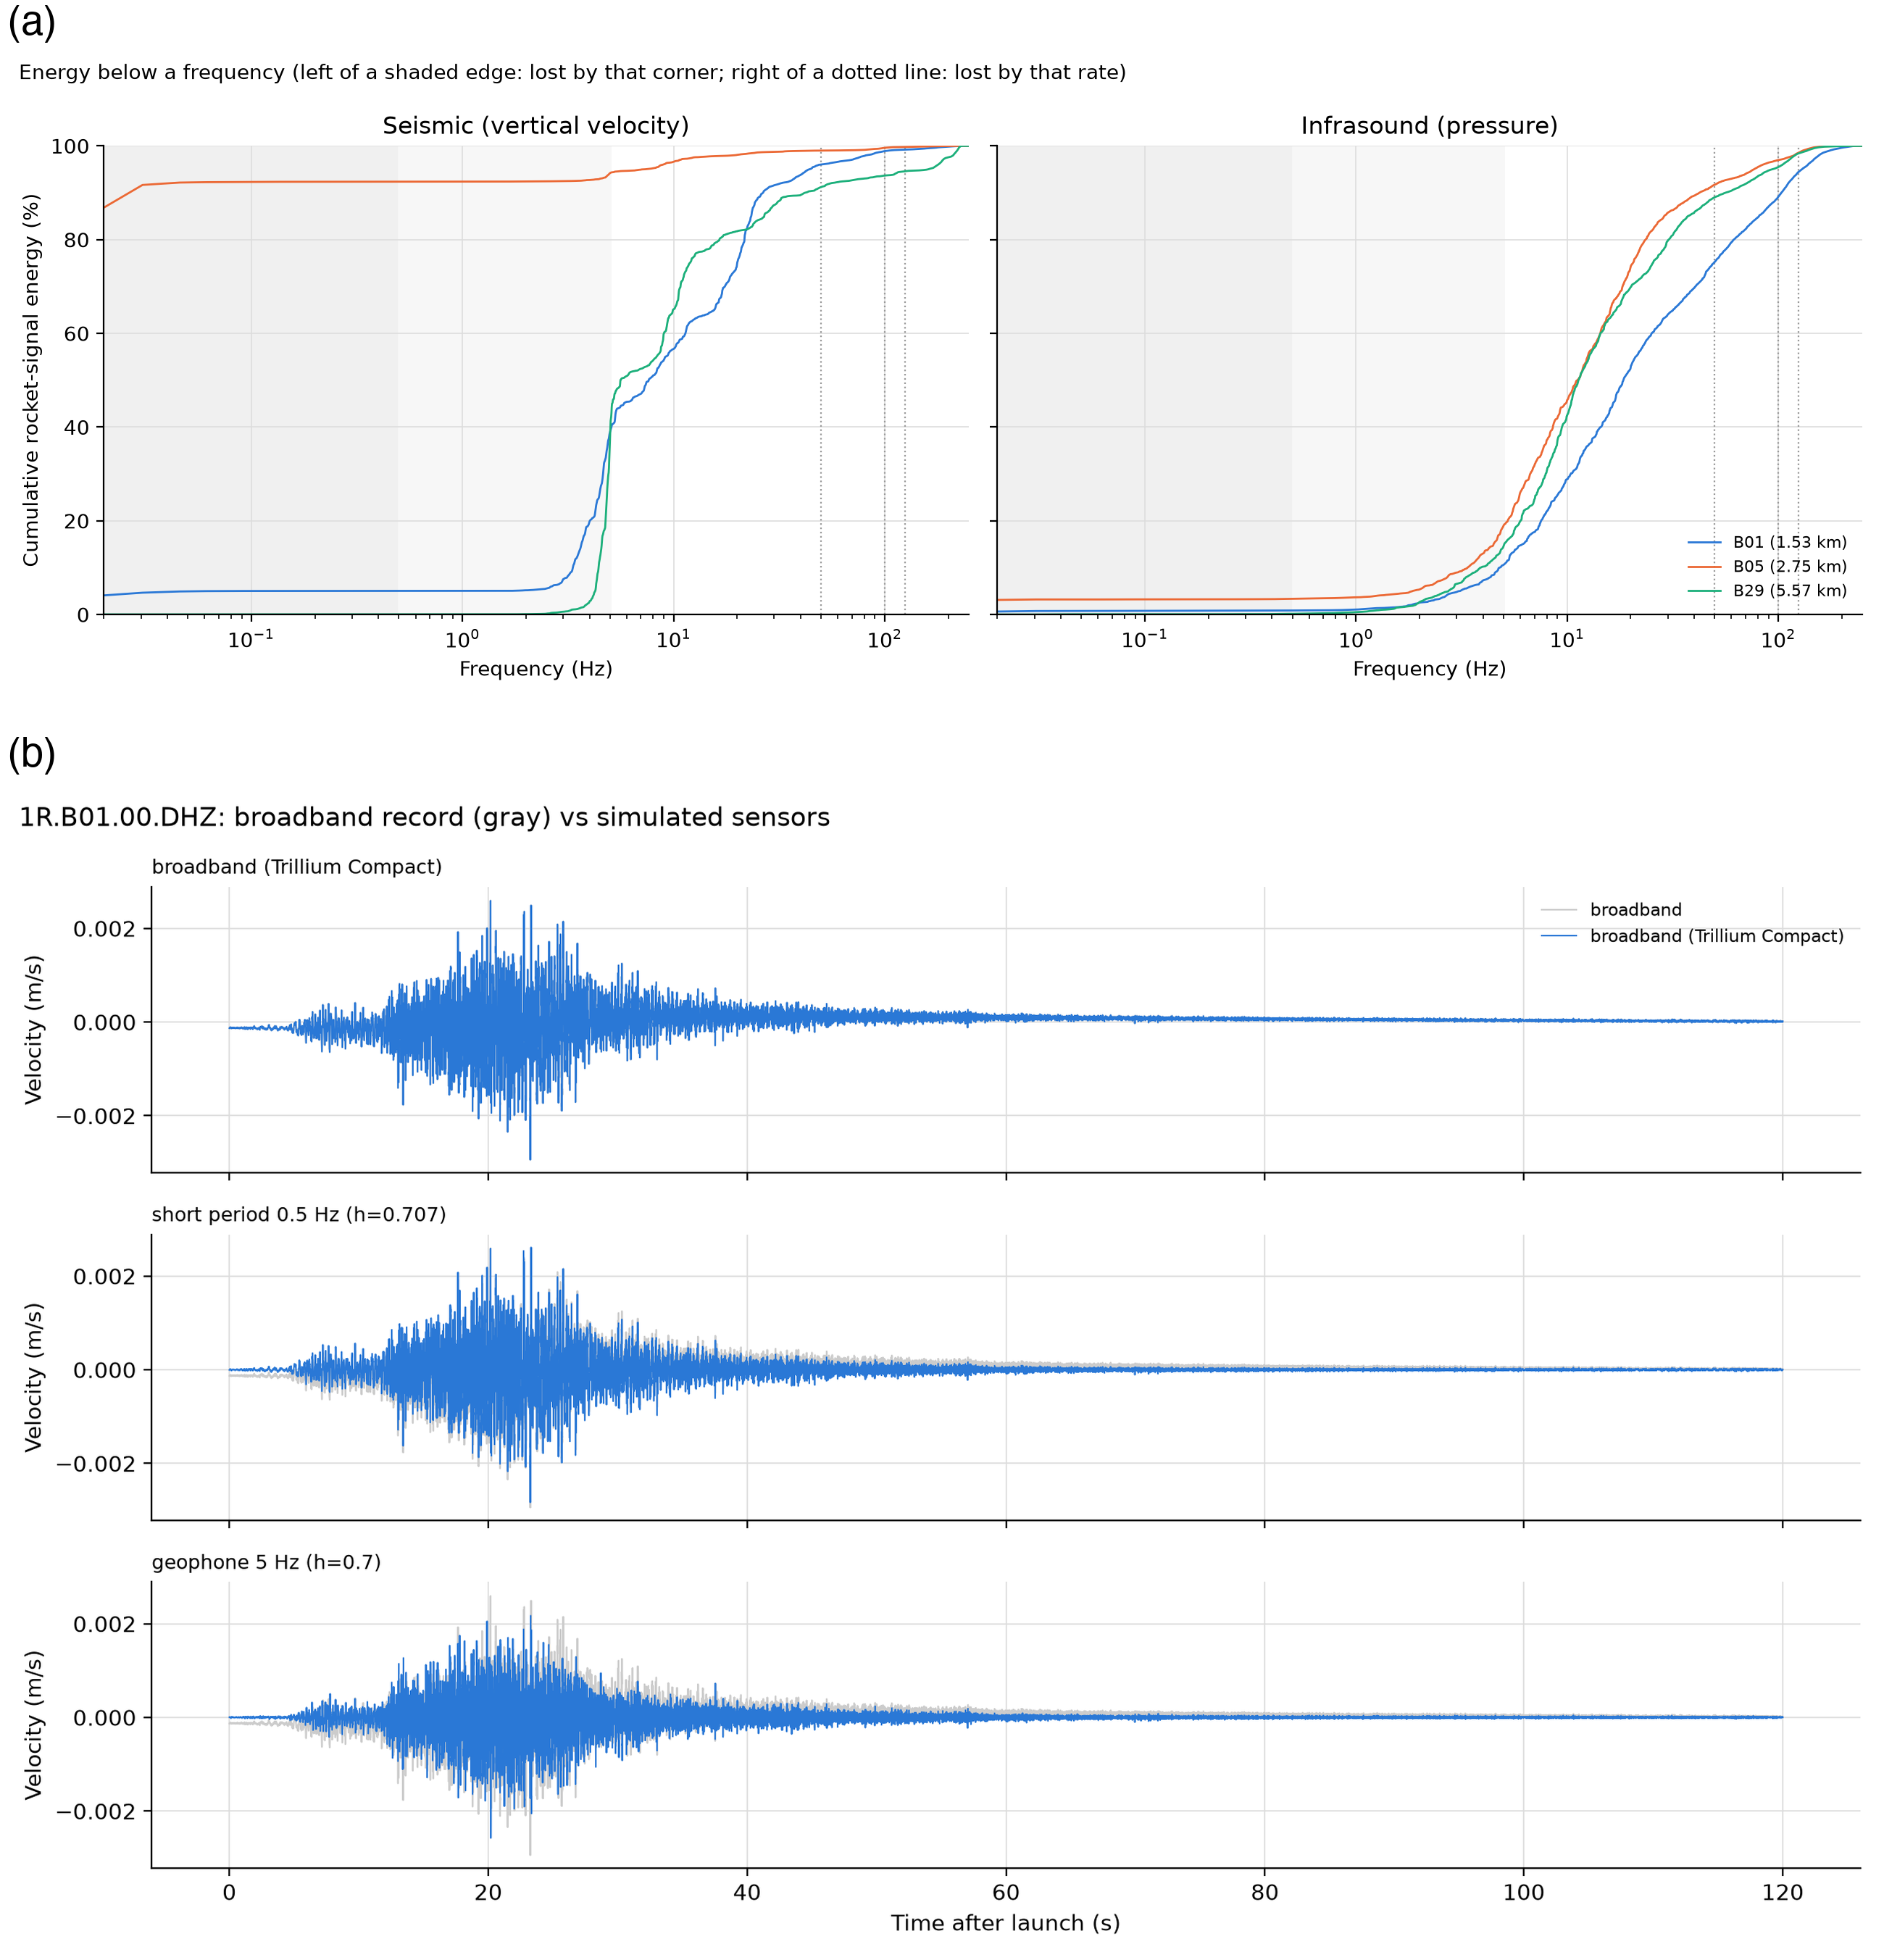
\includegraphics[width=0.9\textwidth]{composite_bandwidth}
  \caption{(a) Cumulative share of rocket-signal energy (launch minus noise
    PSD) below each frequency for vertical velocity (left) and pressure
    (right) at B01, B05 and B29. Shading: below 0.5~Hz and 0.5--5~Hz (energy
    lost by sensors with those corners). Dotted lines: Nyquist frequencies of
    100, 200 and 250~samples~s$^{-1}$ (energy to their right is lost at that
    rate). The B05 seismic curve is dominated by instrument drift below
    0.05~Hz. (b) B01 vertical velocity as recorded by the Trillium Compact and
    as a 0.5~Hz short-period sensor and a 5~Hz geophone would have recorded
    it (broadband record repeated in gray).}
  \label{fig:bandwidth}
\end{figure}

\subsection{Sensor Corner Frequency}

To test what different seismometers would have recorded, we passed
the Trillium velocity records through the responses of a 0.5~Hz and a
1~Hz short-period sensor and a 5~Hz geophone (Figure~\ref{fig:bandwidth}b).
A 0.5~Hz sensor retains 96--100\% of the peak and 85--100\% of the
energy; what it removes is mostly noise, plus, at B01, a small rise
below 0.2~Hz that may be tilt. A 5~Hz geophone loses real rocket signal:
31--38\% of the energy and 12--14\% of the peak, because the launch
spectrum has a pronounced peak at 4--5~Hz at both stations. Nodal
geophones are therefore adequate for peak amplitudes and timing but
underestimate low-frequency ground motion unless corrected
(Section~\ref{sec:nodal_validation}).

\subsection{Implications for Network Design}

For launch recording at these distances, 250~samples~s$^{-1}$ is
sufficient for ground motion and nearly sufficient for pressure;
pressure within $\sim$3~km of a heavy-lift launch benefits from
500~samples~s$^{-1}$ and from at least 24-bit resolution, since 16-bit
loggers at high gain overflow above $\sim$100~Pa. Seismometers with
corners at or below 1~Hz capture essentially all of the rocket's ground
motion. A low-gain setting, or a co-located higher-range sensor, would
have avoided the Gem overflow within 3.4~km.


%% ============================================================
\section{Air-to-Ground Coupling}
\label{sec:coupling}

At 12 sites a pressure sensor and a vertical seismometer were
co-located, giving 15 sensor pairs: infraBSU and Trillium at B01, B03, B05 and B29
(500~samples~s$^{-1}$) and a Gem and a SmartSolo at the nodal sites
(100~samples~s$^{-1}$). For each pair we computed, over the first 180~s
with Gem overflow intervals masked, the RMS ratio of vertical velocity to
pressure in the 1--40~Hz band, the least-squares regression coefficient
$k$ in $v = k\,p$ at the best lag, and the transfer function
$H(f) = P_{pv}/P_{pp}$ with its coherence and phase from Welch spectra
using only segments free of overflow (Table~\ref{tab:coupling},
Figures~\ref{fig:coupling_tf} and \ref{fig:coupling_summary}).

RMS coupling ratios are 3--11~\si{\micro\metre\per\second\per\pascal}
at all sites with working sensors, with no systematic trend with
distance. The coherent part of the coupling, $|H|$ where coherence
exceeds 0.5, is $\lesssim$1~\si{\micro\metre\per\second\per\pascal} at
1--5~Hz and 1.5--11~\si{\micro\metre\per\second\per\pascal} at 5--40~Hz,
increasing with frequency at most sites. The phase of $H$ at the
Trillium sites is close to 180$^{\circ}$ at 5--20~Hz ($-170^{\circ}$ at
B01, $157^{\circ}$ at B29), so the ground moves down under compression,
as expected for local loading of a compliant surface. Coherence is
moderate (0.1--0.7 at 5--20~Hz), and the RMS ratios exceed the coherent
$|H|$, so a substantial part of the ground motion is not explained by
the local pressure: it includes seismic energy coupled into the ground
elsewhere, notably near the pad. At the B20 sites, ground motion
precedes the air wave, and in the first $\sim$20~s the ratio reaches
16--135~\si{\micro\metre\per\second\per\pascal}; it falls to
8--21~\si{\micro\metre\per\second\per\pascal} when the air wave arrives
and to $\sim$6~\si{\micro\metre\per\second\per\pascal} (median) after
60~s (\suppfig{5}). The two independent instrument pairs at B01
(infraBSU with Trillium and with SmartSolo) give identical coupling
magnitudes with opposite sign, confirming the SmartSolo polarity
reversal.

These coupling magnitudes are broadly consistent with values reported
for controlled explosions and volcanic eruptions at comparable distances.
\citet{thompson_amos6_2026} measured a broadband median seismic/acoustic
coupling coefficient of $2.3\times10^{-6}$~(m~s$^{-1}$)~Pa$^{-1}$ at
the BCHH array approximately 1.4~km from SLC-40 during the 2016 Falcon~9
failure, with frequency-dependent peaks near 4--5 and 20--24~Hz, consistent
with the frequency dependence observed here. \citet{novoselov_ground_coupling_2020}
characterise the coupling efficiency in terms of near-surface properties;
the increase of $|H|$ with frequency at most Artemis~II sites is
consistent with their framework. The partitioning of radiated energy
between acoustic and seismic channels is discussed by
\citet{johnson_aster_2005} in the volcanic context and by
\citet{anthony_hunga_coupling_2023} and \citet{macpherson_hunga_coupling_2025}
for the 2022 Hunga Tonga--Hunga Ha'apai eruption; the Artemis~II
coefficients fall within the range spanned by those datasets.

% Written by a notebook; edit the notebook, not this file.
\begin{table}[htbp]
  \centering
  \caption{Air-to-ground coupling at co-located sites, first 180~s after launch. $k_\text{rms}$: RMS ratio of vertical velocity to pressure, 1--40~Hz. $k$: regression coefficient at the best lag ($v = k\,p$; negative means downward motion under compression; SmartSolo signs are as recorded, i.e.\ reversed). $r$: correlation at that lag. $|H|$: median transfer-function magnitude where coherence $\geq$~0.5 (--: none). $\gamma^2$: median coherence, 5--20~Hz. Units \si{\micro\metre\per\second\per\pascal}. B03's Centaur pair is faulty.}
  \label{tab:coupling}
  \scriptsize
  \begin{tabular}{lrrrrrrrr}
  \toprule
  Pair (pressure / velocity) & $r$ (km) & $k_\text{rms}$ & $k$ & corr. & $|H|_{1-5}$ & $|H|_{5-20}$ & $|H|_{20-40}$ & $\gamma^2_{5-20}$ \\
  \midrule
  B14..HDF / B14..DPZ & 0.74 & 4.5 & +1.3 & +0.28 & 0.72 & 2.2 & 8.2 & 0.71 \\
  B01.00.DD0 / B01.00.DHZ & 1.53 & 7.5 & $-$2.6 & $-$0.35 & 0.58 & 5.1 & 7.1 & 0.30 \\
  B01.00.DD0 / B01..DPZ & 1.53 & 7.5 & +2.7 & +0.35 & -- & 5.3 & 7.1 & 0.32 \\
  B01..HDI / B01..DPZ & 1.53 & 5.1 & +1.4 & +0.28 & 0.59 & 3.8 & 5.5 & 0.27 \\
  B03.00.DD0 / B03.00.DHZ & 1.75 & 54.7 & +5.0 & +0.09 & -- & -- & -- & 0.10 \\
  B03..HDI / B03..DPZ & 1.75 & 6.9 & $-$1.4 & $-$0.21 & 1.3 & 2.8 & 3.5 & 0.16 \\
  B12..HDF / B12..DPZ & 2.65 & 9.5 & +3.2 & +0.33 & -- & 11 & 6.4 & 0.41 \\
  B05.00.DD0 / B05.00.DHZ & 2.76 & 3.2 & +0.8 & +0.24 & -- & 1.6 & 2.4 & 0.26 \\
  B07..HDF / B07..DPZ & 3.42 & 6.0 & +1.4 & +0.24 & -- & 2.0 & 1.5 & 0.36 \\
  B24..HDF / B24..DPZ & 5.53 & 7.5 & +2.1 & +0.29 & -- & 5.3 & 6.0 & 0.50 \\
  B23..HDF / B23..DPZ & 5.54 & 9.8 & +2.2 & +0.22 & -- & 3.4 & 3.2 & 0.28 \\
  B29.00.DD0 / B29.00.DHZ & 5.58 & 10.5 & $-$3.0 & $-$0.29 & -- & 5.9 & 6.5 & 0.42 \\
  B20W..HDF / B20W..DPZ & 7.58 & 10.2 & +2.3 & +0.22 & -- & -- & 6.9 & 0.16 \\
  B20..HDF / B20..DPZ & 7.61 & 11.2 & +2.1 & +0.19 & -- & -- & 9.8 & 0.10 \\
  B20S..HDF / B20S..DPZ & 7.63 & 10.4 & +2.3 & +0.22 & -- & -- & 8.2 & 0.13 \\
  \bottomrule
  \end{tabular}
\end{table}
  % written by notebook 65

\begin{figure}[htbp]
  \centering
  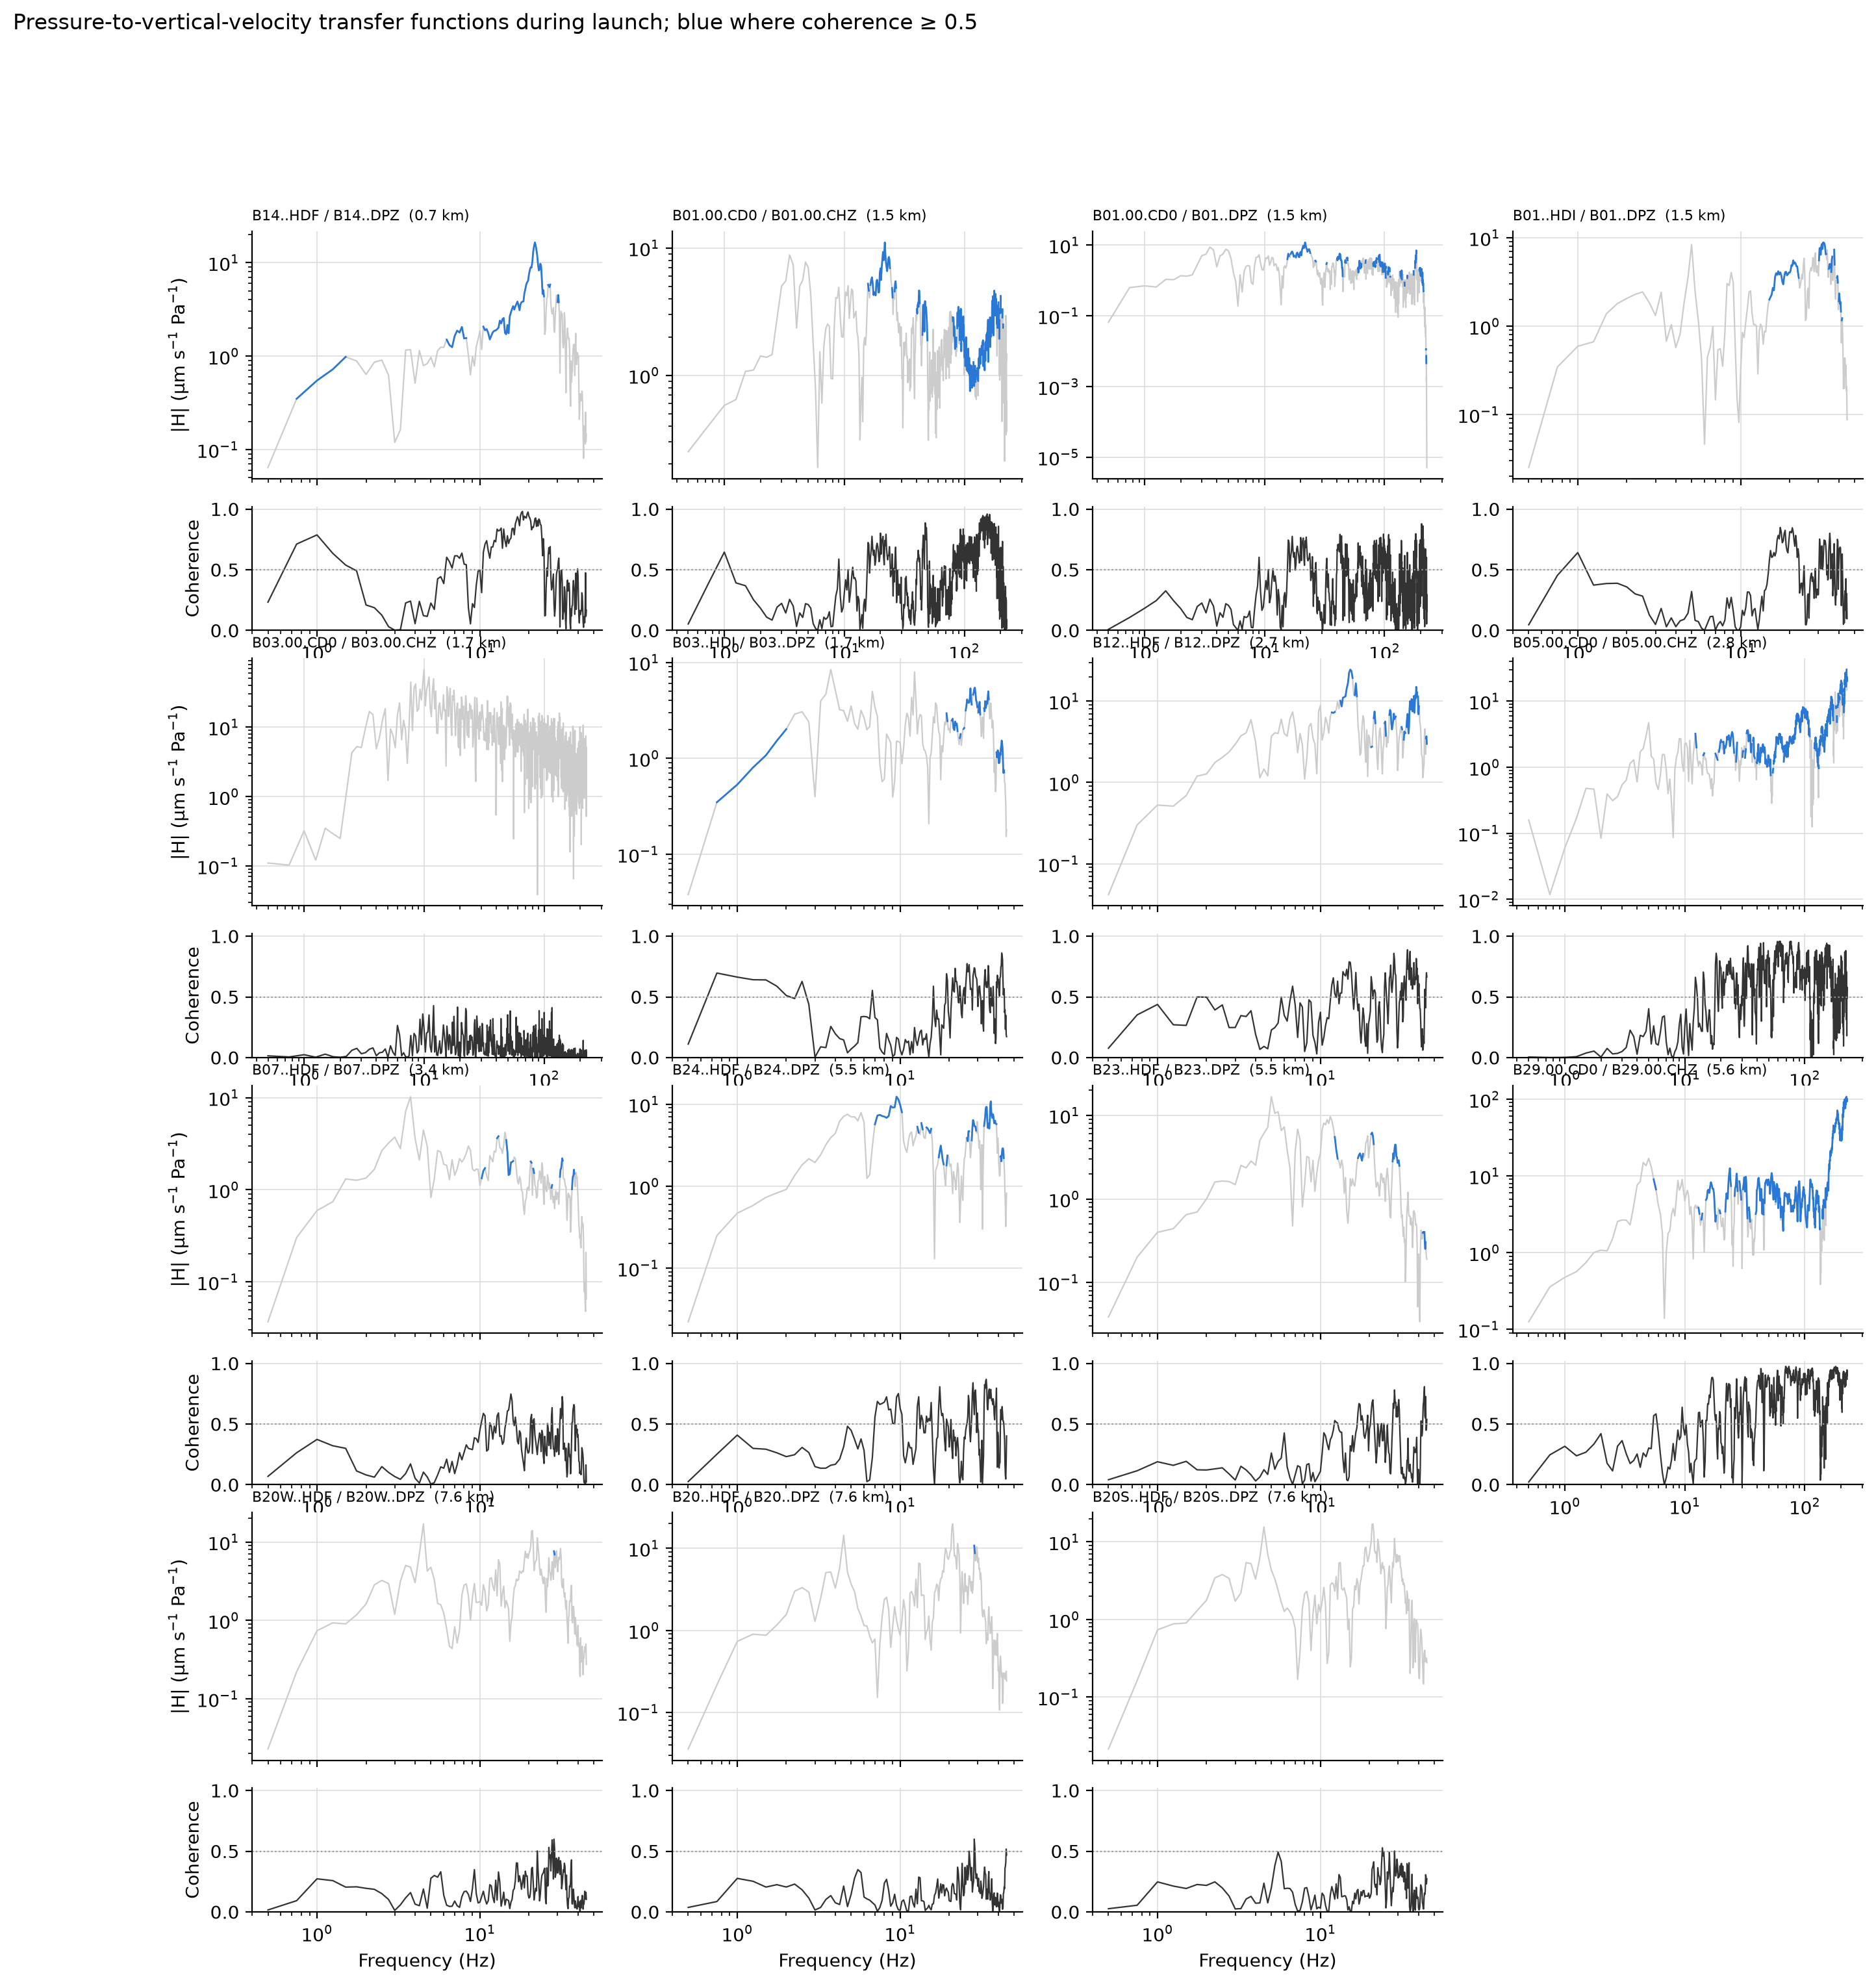
\includegraphics[width=\textwidth]{coupling_transfer_functions}
  \caption{Pressure-to-vertical-velocity transfer-function magnitude
    (top of each panel; blue where coherence $\geq$~0.5) and coherence
    (bottom) at each co-located pair, sorted by distance.}
  \label{fig:coupling_tf}
\end{figure}

\begin{figure}[htbp]
  \centering
  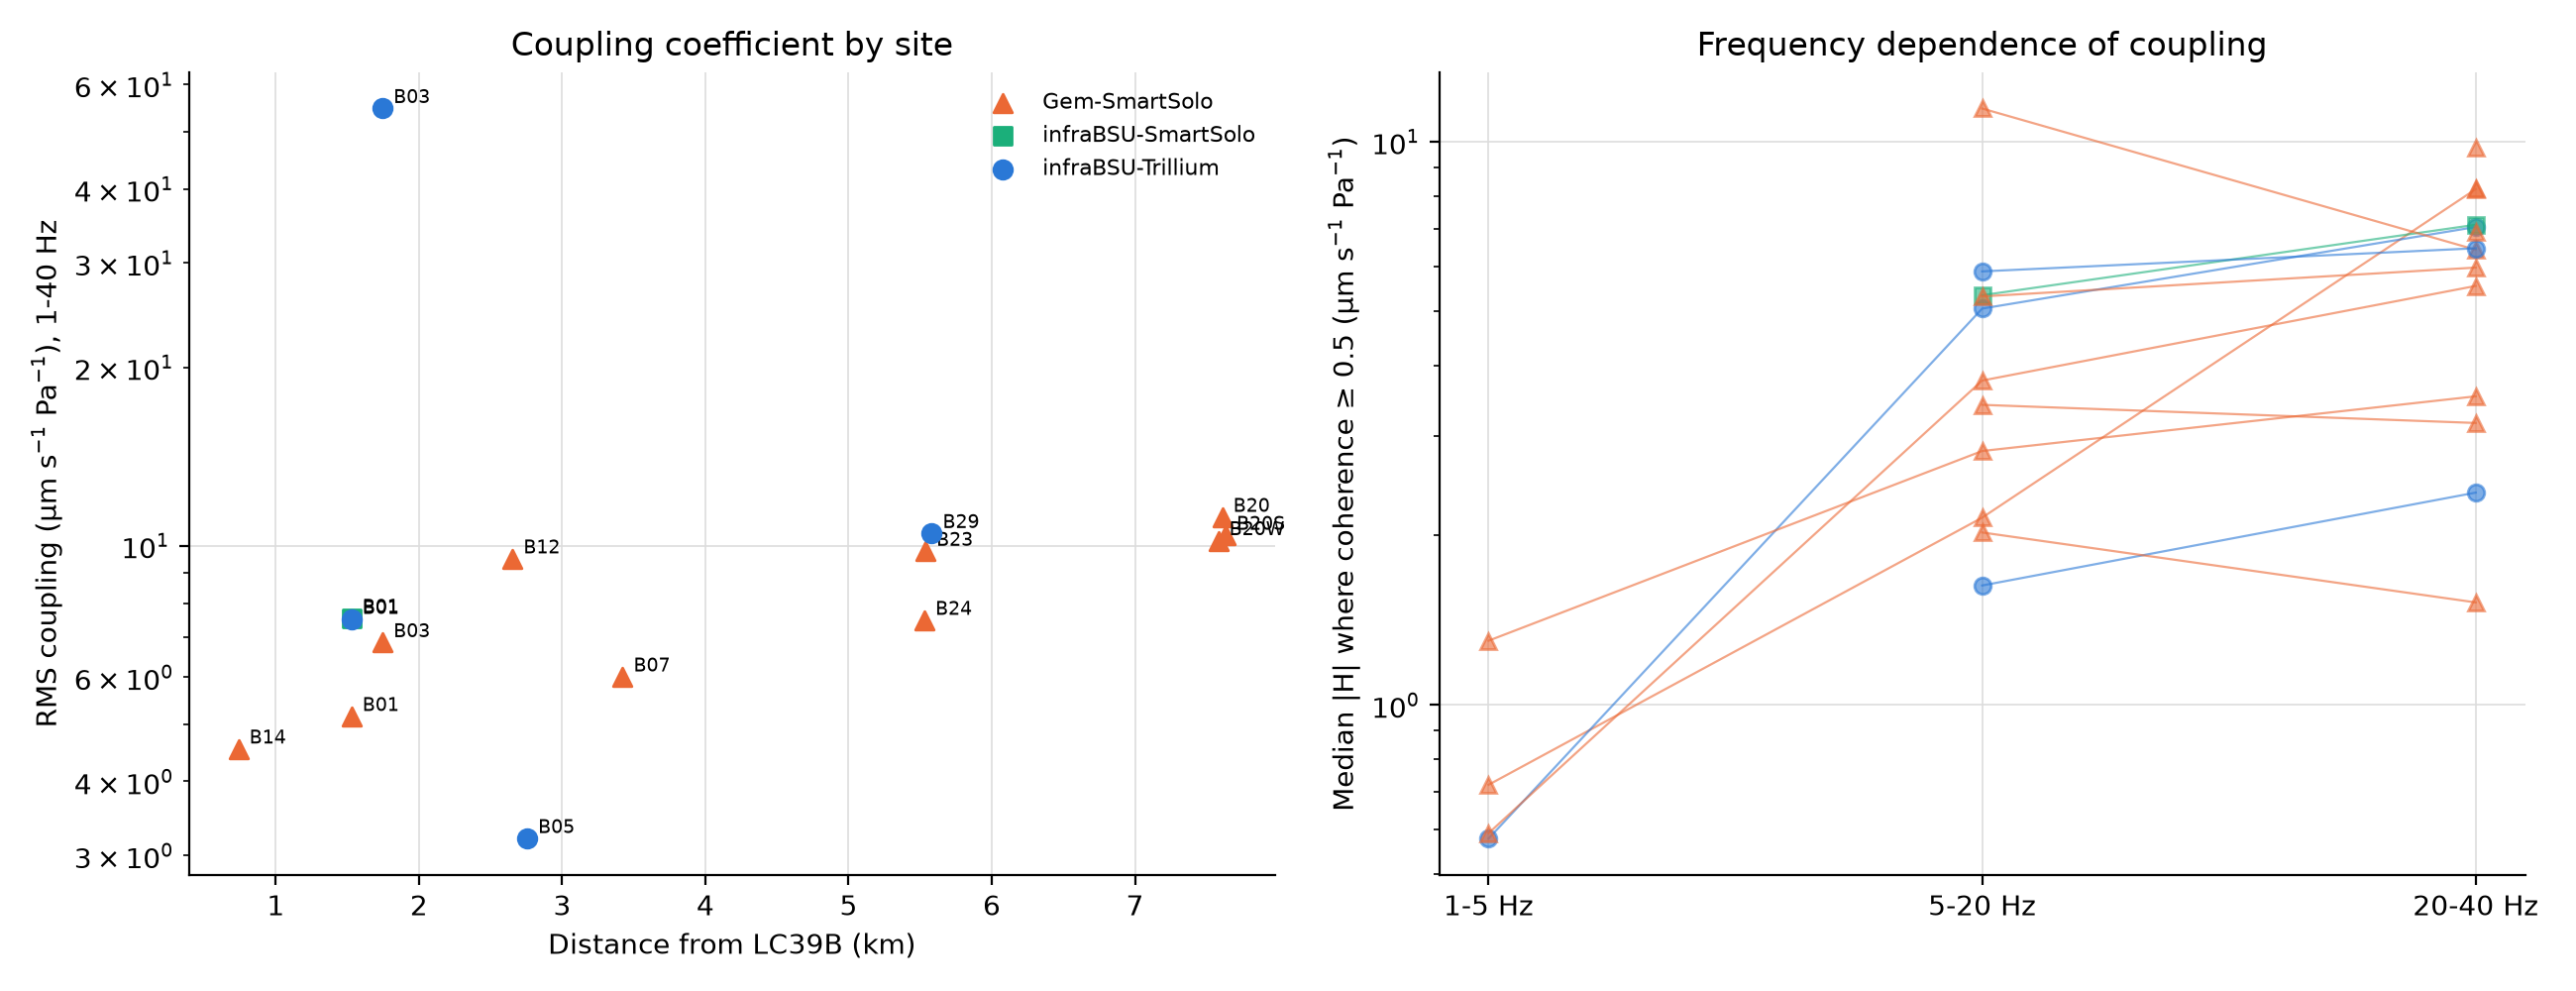
\includegraphics[width=\textwidth]{coupling_summary}
  \caption{Left: RMS coupling ratio (1--40~Hz) by site and instrument
    pair against distance. Right: median coherent transfer-function
    magnitude in three frequency bands.}
  \label{fig:coupling_summary}
\end{figure}


%% ============================================================
\section{Discussion}

\subsection{Recommendations for Launch Deployments}

Rocket signal at 0.7--7.6~km lies above 0.5~Hz in pressure and above
1~Hz in ground motion, so a 0.5~Hz high-pass is appropriate for launch
analyses and sensors with corners at or below 1~Hz capture essentially
all of the rocket's ground motion. 250~samples~s$^{-1}$ suffices for
ground motion; pressure within $\sim$3~km of a heavy-lift launch, and
any analysis of shock fronts or crackle, needs 500~samples~s$^{-1}$.
Sixteen-bit infrasound loggers at high gain overflow above
$\sim$100~Pa, so near-pad sites need 24-bit digitizers, low-gain
settings or a co-located higher-range sensor; where overflow does occur,
it can be detected from the baseline offset it leaves, repaired, and the
record used outside the overflow interval. Protective totes can be used
without correction below $\sim$10~Hz and may reduce wind noise, but their
wall resonances alter the spectrum above $\sim$10~Hz, most densely at
$\sim$20--150~Hz (Text~S1), which matters for sensors recording at
500~samples~s$^{-1}$ inside them. Low-cost 5~Hz nodes are
adequate for peak ground velocity and timing once their response is
removed, but they record voltage rather than velocity and, in this
deployment, with reversed vertical polarity, so both must be checked
before nodal data are combined with broadband data. Co-locating a
pressure sensor with each seismometer is inexpensive and yields the
air-to-ground coupling at every site.

\subsection{Limitations}

The SmartSolo and the infraBSU responses above $\sim$100~Hz are nominal,
the infraBSU records above $\sim$10~Hz include the response of the tote
that housed them (up to $\sim$3~dB at 10--40~Hz at B29, unknown above
50~Hz),
and the polarity of the SmartSolo horizontals was not checked. The
coupling analysis does not separate air-coupled from ground-coupled
seismic energy. Bandwidth conclusions rest on three stations with working
24-bit pressure and seismic sensors, and B05's seismometer was faulty.


%% ============================================================
\section{Conclusions}

The co-located instruments deployed for Artemis~II show what a
heavy-lift launch demands of a recording network. Six 16-bit Gem
channels within 3.4~km of the pad overflowed for 14--29~s above
$\sim$100--140~Pa. Overflow leaves a persistent baseline step that
distinguishes it from shock fronts, and after repair the records outside
the overflow intervals match a co-located 24-bit microbarometer. Tote
enclosures did not change the launch signal below $\sim$10~Hz (peak
ratios 0.94--1.08, coherence $>$0.98 to 45~Hz) but altered the spectrum
above it by up to $\pm$4~dB, depending on the site, and reduced
pre-launch noise at two of three sites. SmartSolo data are geophone
voltage with reversed vertical polarity; once corrected, they agree with
broadband seismometers within 4\%. Rocket signal lies above 0.5~Hz in
pressure and 1~Hz in ground motion. Sampling at 250~samples~s$^{-1}$
suffices for ground motion, but near-pad pressure loses 30\% of its
energy at 100~samples~s$^{-1}$, and a 5~Hz geophone loses a third of the
seismic energy. Air-to-ground coupling is
3--11~\si{\micro\metre\per\second\per\pascal} (RMS, 1--40~Hz),
increases with frequency and corresponds to downward motion under
compression, but is only moderately coherent with the local pressure.
Together these results give a validated dataset for the source analysis
in \papertwo{} and a set of practical requirements for future launch
deployments.


%% ============================================================
\section*{Data and Code Availability}

Waveform data will be archived at EarthScope Data Services
\todo{network codes (1R; MSFC stations?), DOI and release date}. The analysis notebooks, the
\texttt{ksclib} package and \texttt{compose\_figures.py} are available
at \todo{repository URL}, and the version used for this paper is
archived at \todo{archive DOI, e.g.\ Zenodo}. To reproduce the results,
run notebooks 20--60 in order, then notebook 65 (tables), then
\texttt{python compose\_figures.py} (figures). Gem overflow repair uses
\texttt{flovopy.ingest.gem\_overflow} from FlovoPy
\citep{flovopy_2026} \todo{FlovoPy release and DOI that include
\texttt{gem\_overflow}; currently on an unreleased development branch}.
The analysis also uses ObsPy \citep{Beyreuther2010,krischer_obspy_2015}
and \texttt{gemlog} \todo{cite gemlog}. Supplementary Text~S1,
Figures~S1--S5 and Tables~S1--S2 are provided in a separate file.

\begin{acknowledgements}
The SmartSolo instruments were provided by the EarthScope Primary
Instrument Center (EPIC). Gem infrasound nodes were provided by Boise
State University. \todo{Complete acknowledgements: Katherine, Don?,
Robert, John?, others? NASA MSFC. Any grants to acknowledge?}
\end{acknowledgements}

\section*{Author Contributions}

\todo{Complete CRediT author contributions statement.}

%% ============================================================
%% Bibliography style is set by seismica.cls (abbrvnat_seismica_upcasetitle.bst)
\bibliography{artemis2}  %% references go in artemis2.bib

\end{document}
